\newcommand{\institut}{}
\newcommand{\fachgebiet}{Halbleiterbauelemente}
\newcommand{\veranstaltung}{Praktikum Technologie und Bauelemente der Halbleitertechnik}
\newcommand{\pdfautor}{Thomas Kapa (325319), Alona Siebert (303843), Özgü Dogan (326048), Dirk Babendererde (321836)}
\newcommand{\autor}{Thomas Kapa (325 319)\\ Alona Siebert (303 843)\\ \"Ozg\"u Dogan (326 048)\\ Dirk Babendererde (321 836)}
\newcommand{\pdftitle}{Praktikum\ Technologie und Bauelemente der Halbleitertechnik}
\newcommand{\prototitle}{Praktikum Technologie und Bauelemente der Halbleitertechnik}
\newcommand{\aufgabe}{}

\newcommand{\gruppe}{Gruppe 1}
\newcommand{\betreuer}{Betreuer:\\ Clemens Helfmeier\\ Philipp Scholz}



\input{../../packages/tu_header_9}

\setcaptionwidth{7.5cm}

\begin{document}


% \lstinputlisting{./praktikum6.sce}

\sloppy



%---------------------------------------------------------------------
%---------------------------------------------------------------------
%---------------------------------------------------------------------
% \part[Herstellung eines pn-Übergangs]{Herstellung eines pn-Übergangs}

\section[Die Herstellungsschritte]{Die Herstellungsschritte}
\subsection[Wafervorbereitung]{Wafervorbereitung}
\subsubsection[Nummerierung]{Nummerierung}

Einige Schritte der Waferherstellung waren bereits schon vor unserem Praktikum durch die betreuenden Labormitarbeiter durchgeführt.

Die an sich runden Wafer haben zwei Flats:  großes tieferes Flat gibt die Kristallrichtung des monokristallinen Wafers an und das kleinere Flat gibt den Dotierstoff an. Die für unser Praktikum verwendeten Wafer haben p-Type Substrat und wurden  mit Bor vordotiert.

Danach wurde jeder Wafer auf der Rückseite nummeriert (s. Abb. \ref{fig:WafRueckseite}). Die Nummern waren 120501, 120502 und 120503.

\begin{figure}[H]
    \centering
        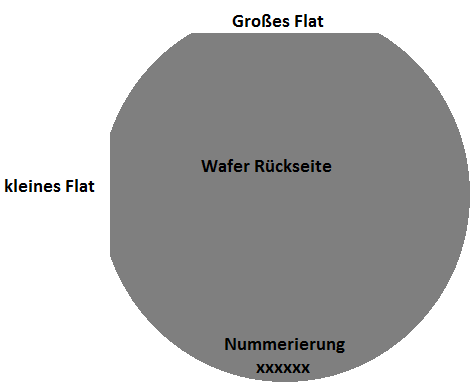
\includegraphics[width=0.4\textwidth]{bilder/WafRueckseite.png}
    \caption{Schema für die Beschriftung}
    \label{fig:WafRueckseite}
\end{figure}


\subsubsection[Reinigung]{Reinigung}

Die Wafer wurden nun vor dem Herstellungsprozess gereinigt. Diesen Schritt brauch man um diverse kleine Partikeln aus der umgebenden Luft, die sich auf der Oberfläche des Wafers ablagern, zu entfernen. Außerdem können metallische Rückstände bei der Nummerierung der Wafer auftreten.
Es wurde ein RCA-Reinigungsprozess verwendet, der aus zwei Schritten besteht: Standard-Clean 1 und Standard-Clean 2 (SC1 \& SC2).

SC1 wird zum Entfernen von organischen Resten verwendet: Wafer wird zehn Minuten lang in einer Lösung,  bestehend aus dem deionisierten Wasser $H_{2}O$, Ammoniak $NH_4$+OH und Wasserstoffperoxid $ H_2O_2 $ im Verhältnis 5 : 1 : 1, gespült .
 Außerdem wurde ein HF-Dip mit 1\%iger Lösung 25 Sekunden lang durchgeführt, um das natürliche Oxid von der Oberfläche zu entfernen.
SC2 wird zum Entfernen von metallischen Resten benutzt. Dafür wird der Wafer mit einer wässrigen Lösung aus Salzsäure und Wasserstoffperoxid  im Verhältnis 6 : 1 : 1 behandelt.

Dabei  soll man unbedingt die Warnhinweise beachten. Da bei der Reinigung verwendete Lösungen sehr gefährlich (sehr giftig und stark ätzend) sein können, muss man unbedingt bei der Arbeit mit diesen Lösungen geeignete Schutzbekleidung und geeignete Schutzhandschuhe tragen. Beim Kontakt mit diesen Lösungen soll man sofort gründlich mit Wasser abspülen und den Arzt konsultieren.


\subsubsection[PECVD]{PECVD}

Nach der Reinigung waren die Wafer mit einer dünnen chemischen Oxidschicht ($SiO_2$)  bedeckt. Da diese Schicht zu dünn ist, wird ein RTP-Prozess (Rapid Thermal Processing) benötigt.  Der Wafer wurde auf ca. 1200°C erhitzt.  Die umgebende Luft reagiert mit den Si-Atomen auf der Oberfläche und es bildet sich dabei eine ca. 60 nm-dicke Siliziumoxid-Schicht. Danach wurde ein PECVD Prozess (Plasma Enhansed Chemical Vapor Deposition) benutzt: Es scheidet sich die Oxidschicht  auf der Oberfläche ab, die 250 nm dick ist.

Bei der PECVD erfolgt die Abscheidung von dünnen Schichten durch eine chemische Aktivierung des Reaktionsprozesses, die durch ein Plasma unterstützt wird.
Für die Schichtbildung werden die Ausgangsstoffe als Gasgemisch in einen Rezipienten eingelassen. Durch erhitztes Plasma werden die Bindungen des Reaktionsgases aufgebrochen und in Radikale zersetzt, die sich auf dem Substrat niederschlagen und dort die chemische Abscheidereaktion bewirken.
 Der PECVD-Prozess lief unter 400°C ab.
 Die Oxiddickenmessung danach ergab ca. 400 nm.

Nach dem PECVD-Prozess wurde noch mal RTP-Tempern benötigt, um das Oxid in das Gitter einzufügen und damit das Oxid an der Oberfläche des Substrats gut haften kann. Bei RTP wurde der Wafer 120 Sekunden  lang auf 1000°C erhitzt.
Die Oxiddickenmessung mit dem Photometer danach ergab ca. 420 nm.


\subsubsection[Lithographie mit der AA-Maske]{Lithographie mit der AA-Maske}

Bei dem lithographischen Prozess wurden die Strukturen für die Diffusion der n-Wannen vorbereitet.
Als erstes werden die Wafer von den möglichen Wasser- und Flüssigkeitsresten befreit. Dafür wird der Wafer 30 min. lang bei 200°C auf einer Heizplatte erhitzt.


\paragraph[HMDS]{HMDS}

Außerdem hilft es ein Haftmittel HMDS (Hexamethyldisilazan) auf den Wafer aufzutragen:
die Wafer werden in eine Vakuumgslocke gelegt, es muss 30 Sekunden lang abgepumpt werden, um das Vakuum zu erzeugen.
HMDS  lagert sich an der Oberfläche des Wafers ab (die Dauer beträgt fünf min.).
Anschließend werden die Wafer  eine Minute lang auf der Heizplatte getrocknet.


\paragraph[Belacken \& Softbake]{Belacken \& Softbake}

Die  Wafer werden auf einen Schleuderapparat gelegt und mit dem AZ 5214  Lack beschichtet. Mit dem Schleuderprogramm werden die Wafer auf 4000 U/min beschleunigt.
Nach der 20-minutigen Pause werden die Wafer bei 90°C zwei min. lang getrocknet, damit der Lack fest wird.



\paragraph[Belichten]{Belichten}
Nun werden die Wafer mit der Active Area Mask  (AA-Maske) abgedeckt und vier Sek. belichtet.


\paragraph[Entwickeln \& Hardbake]{Entwickeln \& Hardbake}

Nach der Belichtung wurde  der Lack in einer Rohm Haas - Lösung 70 Sekunden lang
entwickelt.
Danach wurden alle Wafer auf einer Heizplatte unter 120°C fünf min. lang erhitzt, damit der
restliche Lack gegen Ätzmittel noch resistenter wird.
Die Inspektion mit dem Photometer ergab die Dicke des Photolackes ca.1.9 $\mu$m.


\paragraph[nass-chemisches Ätzen]{nass-chemisches Ätzen}

Mit dem Nass-chemischen Ätzen  werden die Fenster zum Substrat weggeätzt.
Die Wafer wurden in der BHF-Lösung (mit Ammoniumfluorid gepufferte Flusssäure) ca. 6,5 min. gehalten.



\paragraph{Fotolack entfernen}

Der Lack wurde mit  Caro's Etch - Lösung entfernt, indem die Wafer für zehn min. lang in diese Lösung eingetaucht wurden.

Die  untere Abbildung \ref{fig:AusgangsStruktur} zeigt die Struktur, wie wir unsere Wafer als Ausgangsmaterial für unseres Praktikum erhalten haben:

\begin{figure}[H]
    \centering
        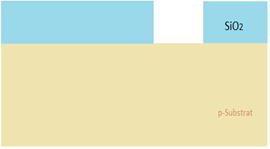
\includegraphics[width=0.5\textwidth]{bilder/AusgangsStruktur.png}
    \caption{Ausgangsstruktur}
    \label{fig:AusgangsStruktur}
\end{figure}

\subsection[Tag 1]{Tag 1}

\subsubsection[Verhaltensregeln in dem Reinraum]{Verhaltensregeln in dem Reinraum}

Als erstes, vor dem Eintritt in den Reinraum, erhielten alle Teilnehmer eine Sicherheitseinweisung vom Herrn Bruhns, dem Laborleiter.
Die Vorschrift ist: Schutzoveralls, spezielle Schuhe, die eine Erdung zum Boden enthalten, und Handschuhe (s. Abb. \ref{fig:Teilnehmer}) zu tragen. Bei der Arbeit mit Chemikalien müssen die Augen zusätzlich geschützt werden. Dazu kann man entweder die Gesichtsschutzmaske oder die Brille
tragen.

Essen und Trinken im Reinraum sind streng verboten.
Außerdem sollte das Verlassen und Wiederbetreten möglichst vermieden werden, da bei jedem Betreten die Partikeln eingeschleppt werden können, die die Reinheit des Labors vermindern.

Weil mit den toxischen Substanzen gearbeitet wird, dürfen die Schwangeren das Praktikum nicht durchführen.

\begin{figure}[H]
    \centering
        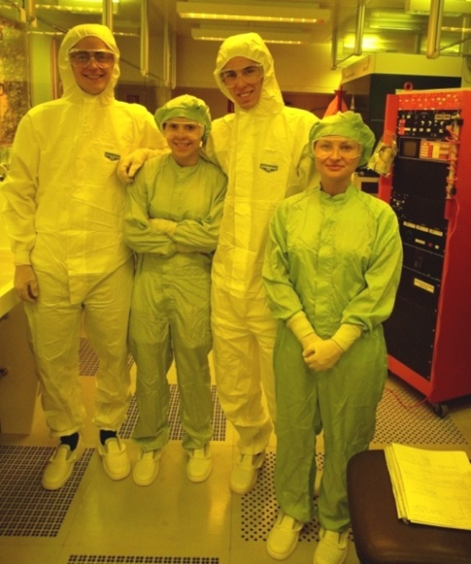
\includegraphics[width=0.5\textwidth]{bilder/Teilnehmer.png}
    \caption{Teilnehmer des Praktikums: Thomas, Özgü, Dirk, Alona}
    \label{fig:Teilnehmer}
\end{figure}

\subsubsection[Dotierstoff aufbringen]{Dotierstoff aufbringen}

Als erstes haben wir unsere drei Wafer unter dem Lichtmikroskop untersucht, um die Struktur der Wafer zu sehen. Da die Oxide das Licht reflektieren, daher ist auch die grüne Farbe im Mikroskop zu sehen (s. Abb. \ref{fig:Mikroskopbild1}) Es wurden keine großen Schäden gefunden.

\begin{figure}[H]
    \centering
        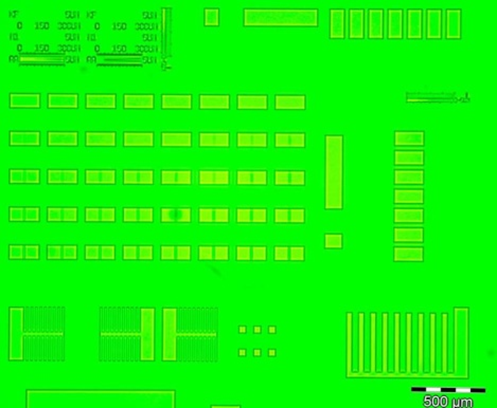
\includegraphics[width=0.35\textwidth]{bilder/Mikroskopbild1.png}
    \caption{Struktur des Wafers}
    \label{fig:Mikroskopbild1}
\end{figure}


Nun wird der Dotierstoff Phosphorus p 509 aufgetragen.


\begin{figure}[H]

\begin{minipage}[hbt]{8cm}
    \centering
    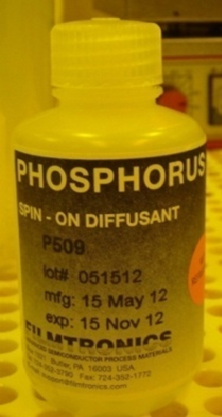
\includegraphics[width=0.35\textwidth, height=5cm]{bilder/Phosphorus.png}
  \caption{Phosphorusflasche}
  \label{fig:Phosphorus}
\end{minipage}
%\hfill
\begin{minipage}[hbt]{6cm}
    \centering
    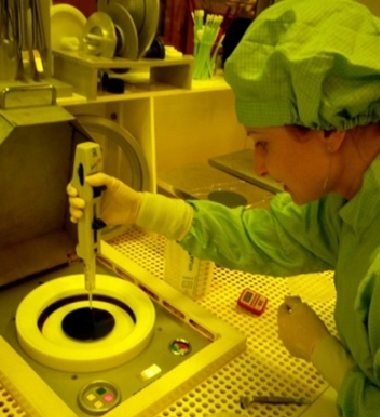
\includegraphics[width=0.8\textwidth,height=5cm]{bilder/Dotierstoffauftragen.png}
  \caption{Dotierstoff auftragen}
  \label{fig:Dotierstoffauftragen}
\end{minipage}

\end{figure}


Um gleichmäßige Verteilung des Dotierstoffes zu bekommen, wurde die Auftragung der Phosphorlösung mit einem Lackschleuderbeschichtungsapparat (s. Abb. \ref{fig:Dotierstoffauftragen}) durchgeführt.
Auf einem Drehtisch wird der Wafer zentral justiert und mittels Vakuum fixiert, damit der Wafer bei der Drehung am Teller gut haftet. Mit Hilfe von Dispenser (der zwei
Mal gedrückt wurde) wird der Dotierstoff auf den Wafer getropft. Danach muss der Wafer sofort in Rotation gebracht werden, um eine ebenmäßige Dotierstoffschicht zu bekommen. Bei der Rotation wird die überflüssige Stoffmenge von der Scheibe weggeschleudert.
Es bleibt nur eine sehr dünne Phosphorschicht auf dem Wafer.

Bedingungen beim Aufschleudern der Phosphorlösung:

\vspace{3mm}


\begin{center}

Programm 4

2500 U/min (Anzeige 250)

2 ml Lösung

\end{center}

\vspace{5mm}
Bemerkung: der Wafer 120503 wurde doppelt mit dem Dotierstoff beschichtet (ca. 4 ml).
Anschließend wurden alle drei Wafer auf der Heizplatte 15 Minuten lang bei 200°C gebacken. Bei diesem Prozessschritt bildet sich ein  Phosphorglas (Silikat). Dabei wurde eine Dampfwolke beobachtet.
Das Ergebnis nach diesem Vorgang ist in der Abbildung \ref{fig:StrukturmitPhosphorus} zu sehen.

\begin{figure}[H]
    \centering
        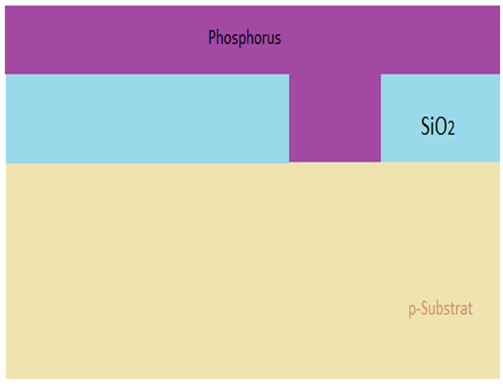
\includegraphics[width=0.5\textwidth]{bilder/StrukturmitPhosphorus.png}
    \caption{Wafer bedeckt mit Phosphorglas}
    \label{fig:StrukturmitPhosphorus}
\end{figure}

Eine Sichtkontrolle mit dem Lichtmikroskop hat uns folgendes ausgegeben (Abb. \ref{fig:Mikroskopbild2}):

Zu beobachten war:
Bei dem Wafer 02 waren Bläschen stärker, der Wafer 03 hatte fast gar keine Bläschen, die Struktur war ebenmäßiger und er enthielt so viel Dotierstoff, dass die Fenster kaum zu sehen waren. Der Wafer 01 hatte große Bläschen, die ständig Ihre Form verändert haben (Abb. \ref{fig:Mikroskopbild2}).

\begin{figure}[H]
    \centering
        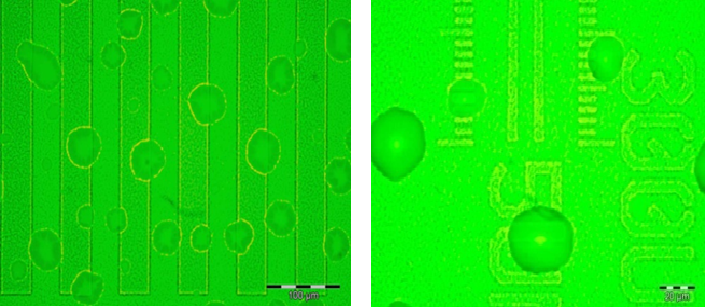
\includegraphics[width=0.7\textwidth]{bilder/Mikroskopbild2.png}
    \caption{Lichtmikroskopbild, Wafer01}
    \label{fig:Mikroskopbild2}
\end{figure}

\subsubsection[Diffusionsofen]{Diffusionsofen}

Jetzt kommen die Wafer in den Diffusionsofen.

Als erstes wurden die Wafer  so in dem Quarzschiffchen (Abb. \ref{fig:Quarzschiffchen}) einsortiert, dass sich die Vorderseiten der Wafer 01 und 02 gegenüber stehen. Wafer 03 wurde einsam auf der anderen Seite des Quarzschiffchens platziert.

\begin{figure}[H]
\centering
\begin{minipage}[hbt]{6cm}
    \centering
    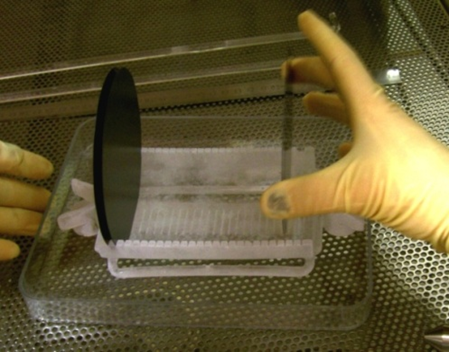
\includegraphics[width=1\textwidth, height=4cm]{bilder/Quarzschiffchen.png}
  \caption{Quarzschiffchen}
  \label{fig:Quarzschiffchen}
\end{minipage}
%\hfill
\begin{minipage}[hbt]{7cm}
    \centering
    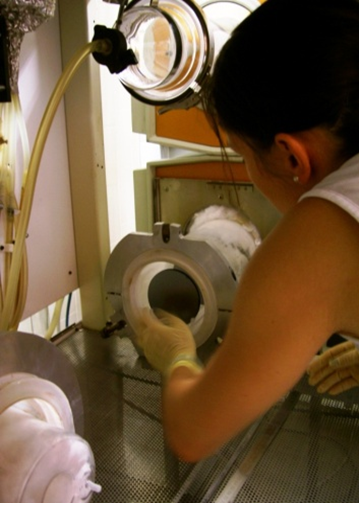
\includegraphics[width=0.7\textwidth,height=6cm]{bilder/einbringeninDiffusionsofen.png}
  \caption{Einbringen in den Diffusionsofen}
  \label{fig:einbringeninDiffusionsofen}
\end{minipage}

\end{figure}

Dann wird das Schlitten 65 cm tief im Ofen platziert, damit die Wafer sich möglichst in der Ofenmitte befinden.
Zum Abschluss wurde anschließend noch ein Quarzhohlzylinder in den Ofen (Abb. \ref{fig:einbringeninDiffusionsofen}) geschoben, um die Temperaturhaltung zu verbessern.
Der Prozess der Diffusion findet unter dem Durchströmen des Diffusionsofens (Abb. \ref{fig:diffusionsofen}) mit dem Prozessgas für zehn min. bei der Temperatur von 1000°C.

\begin{figure}[H]
    \centering
        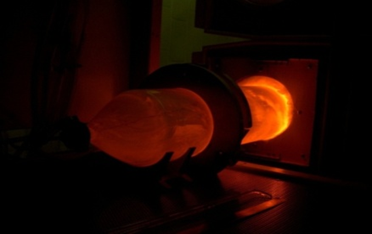
\includegraphics[width=0.4\textwidth]{bilder/diffusionsofen.png}
    \caption{Diffusionsofen}
    \label{fig:diffusionsofen}
\end{figure}

Nach dem Diffusionsprozess verblieben die Wafer noch zum langsamen Auskühlen über die Nacht im Ofen.

Nach der Diffusion sieht unsere Struktur so aus (Abb. \ref{fig:StrukturnachDiffusionsofen}):

\begin{figure}[H]
    \centering
        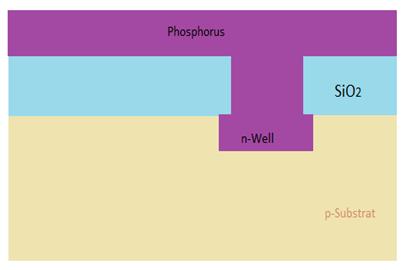
\includegraphics[width=0.5\textwidth]{bilder/StrukturnachDiffusionsofen.png}
    \caption{Struktur nach dem Diffusionsofen}
    \label{fig:StrukturnachDiffusionsofen}
\end{figure}


\subsection[Tag 2:]{Tag 2:}


Am zweiten Tag haben wir unsere Wafer aus dem Ofen genommen. Dabei haben wir beobachtet, dass der Wafer 03 glänzend und der Wafer 01 und 02 matt waren. Danach wurden alle Wafer einer Sichtkontrolle unter dem Mikroskop unterzogen und  mit dem Photometer wurde die Schichtdicke gemessen.


\subsubsection[Sichtkontrolle]{Sichtkontrolle}

\paragraph[Photometer]{Photometer}

Das Photometer Ergolux (Abb. \ref{fig:Photometer}) besteht aus einem Mikroskop mit einem
Aufsatz, der Licht bestimmter Wellenlängen (zwischen 400 nm und 800 nm ) auf den Wafer strahlt und über die Reflexion der Lichtquanten der unterschiedlichen Wellenlängen den Aufschluss über die Schichtdicke gibt.

Zur Kalibrierung muss das Photometer mit einer Musterprobe justiert werden(mit dem Flat nach unten):  die Musterprobe (ein nicht beschichteter Siliziumwafer) soll auf den Objekthalter so platziert werden, damit man die Bildschärfe einstellen kann. Dann startet man das Programm  Justage. Danach wird es ohne Musterprobe auf dem Objekthalter noch mal gestartet.
Nur dann  können wir unsere Wafer messen.

Die Messergebnisse für unsere drei Wafer sind in der Tabelle \ref{tab:gemessene Phosphorglasdicke in nm} unten zusammengefasst.

\begin{table}[H]
\centering
\caption{gemessene Phosphorglasdicke in nm}
\begin{tabular}{|c|c|c|c|c|c|}

       \hline
       Wafer  & oben & mittig & unten & links & rechts \\
        \hline
       120501       & 82.3 &    78.1 &  86.8 &  85.4    & 73.2        \\
        \hline
       120503     & 770.1   & 784.8 &   765.3   & 764.8 & 776.2        \\
        \hline

\end{tabular}
\label{tab:gemessene Phosphorglasdicke in nm}
\end{table}


Die Wafer 01 und 02 waren nicht gut messbar! Der Wafer 03  hat dagegen fast perfekte Messergebnisse \ref{fig:Photometerbild}.

\begin{figure}[H]
\centering
\begin{minipage}[hbt]{6cm}
    \centering
    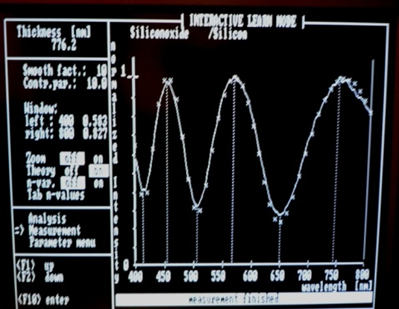
\includegraphics[width=1\textwidth, height=4cm]{bilder/Photometerbild.png}
  \caption{Photometermessung}
  \label{fig:Photometerbild}
\end{minipage}
%\hfill
\begin{minipage}[hbt]{7cm}
    \centering
    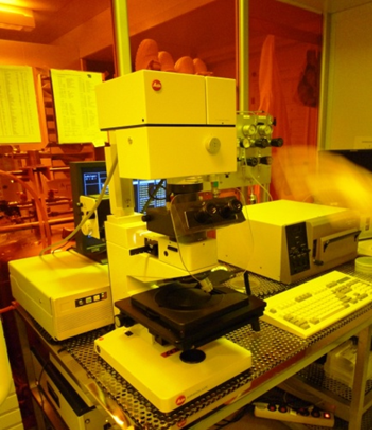
\includegraphics[width=0.7\textwidth,height=6cm]{bilder/Photometer.png}
  \caption{Photometer}
  \label{fig:Photometer}
\end{minipage}

\end{figure}



\paragraph[Sichtkontrolle unter dem Lichtmikroskop ]{Sichtkontrolle unter dem Lichtmikroskop }
Wafer02 (Abb. \ref{fig:MikroskopW2}) und Wafer01 (Abb. \ref{fig:MikroskopW1}):keine klare Struktur(wegen sehr guten Diffusion??)


\begin{figure}[H]
\centering
\begin{minipage}[hbt]{6cm}
    \centering
    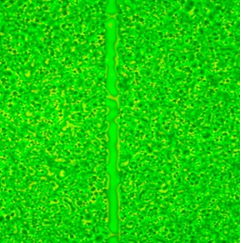
\includegraphics[width=0.8\textwidth, height=5cm]{bilder/MikroskopW1.png}
  \caption{Lichtmikroskopbild Wafer01}
  \label{fig:MikroskopW1}
\end{minipage}
%\hfill
\begin{minipage}[hbt]{6cm}
    \centering
    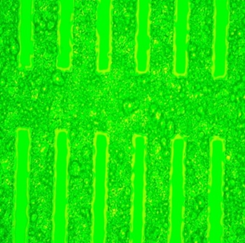
\includegraphics[width=0.8\textwidth,height=5cm]{bilder/MikroskopW2.png}
  \caption{Lichtmikroskopbild Wafer02}
  \label{fig:MikroskopW2}
\end{minipage}

\end{figure}

Wafer03: man kann einen großen Farbunterschied sehen. Die Schicht machte optisch einen guten Eindruck, die Struktur ist sehr klar.


\subsubsection[Ätzen (Entfernen des Phosphorglases)]{Ätzen (Entfernen des Phosphorglases)}

Jetzt wird das Phosphorglas entfernt. Dazu wird zuerst der Wafer01 in die 2.5\%-ige Flusssäure für ca. fünf Minuten lang eingetaucht, um das Phosphorglas von der
Oberfläche zu entfernen. Übrig bleibender Phosphor wurde anschließend mit dem
Wattestäbchen entfernt und in Di-Wasser gesäubert.
Da die Flusssäure stark ätzend ist, müssen ein extra dicker Schutzanzug, Augenschutz und dickere Handschuhe getragen werden (Abbildung \ref{fig:Schutzbekleidung}). Nach dem Ätzen prüften wir die Dicke mit dem Photometer und stellten fest, dass wir die ganze Schicht wegätzten!! Die Sichtkontrolle mit dem Lichtmikroskop \ref{fig:ArbeitenamLichtmikroskop} zeigte, dass Struktur noch da war, deswegen wurde entschieden den Wafer02 für Schrägschliff zu verwenden.


\begin{figure}[H]
\centering
\begin{minipage}[hbt]{7cm}
    \centering
    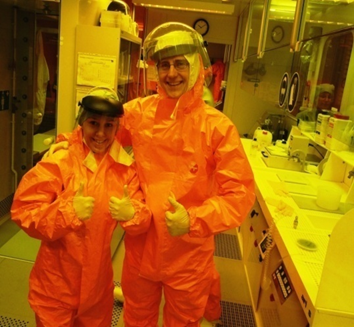
\includegraphics[width=0.9\textwidth, height=6cm]{bilder/Schutzbekleidung.png}
  \caption{Schutzbekleidung}
  \label{fig:Schutzbekleidung}
\end{minipage}
%\hfill
\begin{minipage}[hbt]{7cm}
    \centering
    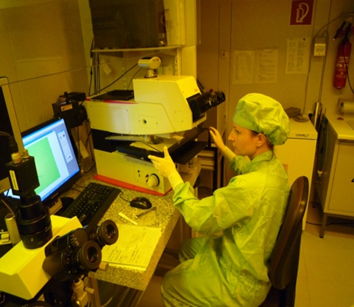
\includegraphics[width=0.9\textwidth,height=6cm]{bilder/ArbeitenamLichtmikroskop.png}
  \caption{Am Lichtmikroskop}
  \label{fig:ArbeitenamLichtmikroskop}
\end{minipage}

\end{figure}


Der Wafer02 wurde dann zwei Mal geätzt: ein Mal sehr vorsichtig mit der 2.5\%-igen Flusssäure nur für eine Minute und danach mit der 1\%-igen nur für fünf Sekunden, jedes Mal wurde die Dicke gemessen.
Der Wafer03 wurde  schon mehrmals  geätzt: zwei Mal sehr vorsichtig mit der 1\%-igen Flusssäure für eine Minute, dann mit der 1\%-igen nur für fünf Sekunden.  Jedes Mal wurde die Dicke kontrolliert. Die Ergebnisse der Oxiddickenmessung sind in der Tabelle \ref{tab:Oxiddickenmessung nach dem Aetzen} dargestellt.

\begin{table}[H]
\centering
\caption{Oxiddickenmessung nach dem Ätzen}
\begin{tabular}{|c|c|c|c|c|c|}

       \hline
       Wafer  & oben & mittig & unten & links & rechts \\
        \hline
       120502       & 196.5 & 199.9 & 198   & 205 & 195        \\
        \hline
       120503     & 201 & 202   & 203.7 & 186.7 & 203        \\
        \hline

\end{tabular}
\label{tab:Oxiddickenmessung nach dem Aetzen}
\end{table}

Nach dem Ätzen sieht unsere Struktur folgendermaßen aus \ref{fig:StrukturnachdemAetzen}:

\begin{figure}[H]
    \centering
        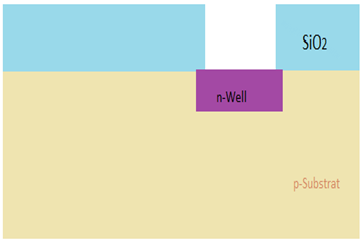
\includegraphics[width=0.5\textwidth]{bilder/StrukturnachdemAetzen.png}
    \caption{Struktur nach dem Ätzen}
    \label{fig:StrukturnachdemAetzen}
\end{figure}
Anschließend wurden die Wafer mit dem Stickstoff trocken gepustet und für ca. 15 min. bei 200°C auf eine Heizplatte gelegt, um die molekulare Flüssigkeitsreste von der Oberfläche des Wafers zu entfernen (sie stören die Haftung des Photolacks).




\subsubsection[Lithographie mit der KF-Maske]{Lithographie mit der KF-Maske }

\paragraph[HMDS ]{HMDS}

Die Wafer 02 und 03 werden direkt von der Heizplatte \ref{fig:Heizplatte} in Exikator, eine so
genannte Vakuumglocke(s. Abb \ref{fig:Vakuumglocke}) mit dem  Haftmittel HMDS (Hexamethyldisilazan), gebracht.


\begin{figure}[H]
\centering
\begin{minipage}[hbt]{6cm}
    \centering
    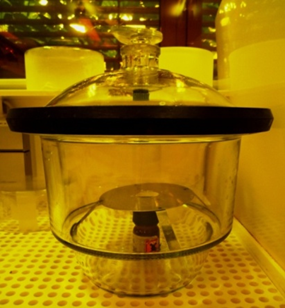
\includegraphics[width=0.9\textwidth, height=6cm]{bilder/Vakuumglocke.png}
  \caption{Vakuumglocke}
  \label{fig:Vakuumglocke}
\end{minipage}
%\hfill
\begin{minipage}[hbt]{6cm}
    \centering
    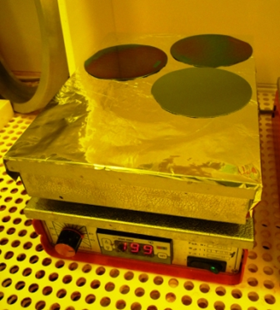
\includegraphics[width=0.9\textwidth,height=6cm]{bilder/Heizplatte.png}
  \caption{Heizplatte}
  \label{fig:Heizplatte}
\end{minipage}

\end{figure}



Es wird das Vakuum für 30 Sekunden lang abgepumpt, HMDS verdampft und lagert sich an der Oberfläche des Wafers ab. Es wird ca. fünf Minuten beschichtet, danach wird das Druckventil sehr langsam gedreht und der Druck abgelassen. Anschließend werden die Wafer für eine Minute bei 120°C auf die Heizplatte gelegt.



\paragraph[Belacken und Softbake]{Belacken und Softbake}

Nachdem die Wafer getrocknet waren, wurden sie mit einem Positivlack AZ 5214 beschichtet (s.Abb \ref{fig:BeschichtungdesWafers} und \ref{fig:Lackflasche}).
Beim Drehen der Schleuder, wenn sich der Lack ausbreitet, beobachtet man die farbigen Wellen. Es sind die Interferenzwellen von den Lackschichten. Je länger die Schleuderzeit ist, desto gleichmäßiger ist die Lackschicht.

\begin{figure}[H]
\centering
\begin{minipage}[hbt]{6cm}
    \centering
    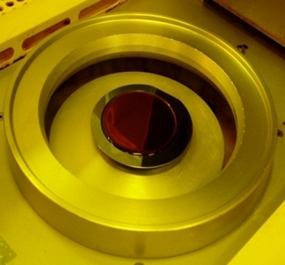
\includegraphics[width=0.9\textwidth, height=5.5cm]{bilder/BeschichtungdesWafers.png}
  \caption{Waferbeschichtung}
  \label{fig:BeschichtungdesWafers}
\end{minipage}
%\hfill
\begin{minipage}[hbt]{6cm}
    \centering
    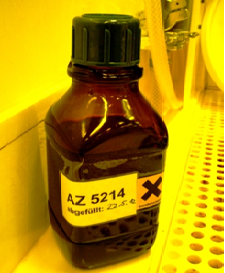
\includegraphics[width=0.9\textwidth,height=5.5cm]{bilder/Lackflasche.png}
  \caption{Lackflasche}
  \label{fig:Lackflasche}
\end{minipage}

\end{figure}




Nach dem Lackieren muss der Wafer 30 Minuten lang in der halboffenen Schachtel
ruhen, damit die Gasbläschen rauskommen und der Lack in die kleinsten Rauigkeiten der
Oberfläche eindringen kann.
Anschließend wurden die Wafer bei 90°C zwei Minuten auf der Heizplatte erhitzt, um
den Lack zu fixieren. Sehr wichtig, dass die Wafer sich sehr langsam abkühlen müssen!


\paragraph[Belichten mit der KF-Maske ]{Belichten mit der KF-Maske}

Das Belichten des Wafers erfolgt auf dem Belichtungsapparat:

Dieser Lithographie-Apparat hat die Belichtungshaube, darunter ist der Waferhalter und Maskenhalter(s.Abb. \ref{fig:Maskenjustierer}),  Mikroskop mit einer CCD-Kamera und einem Bildschirm.
Ganz wichtig ist es, dass die Maske und der Wafer genau übereinander liegen, damit der
Wafer an den nötigen Stellen belichtet werden kann.
 Als erstes wurde Maskenjustierer angeschaltet und die Lampe vorgewärmt. Auf dem Bildschirm kann man die unten erscheinenden Anleitungen befolgen. Weiter wurde die Maske geladen und mit dem Vakuum festgehalten. Die KF-Maske wurde genau an der AA-Maske justiert(man kann die Justierung in der Abbildung \ref{fig:Justiervorgang} sehen, wo die Kreuze übereinanderliegen).

\begin{figure}[H]
\centering
\begin{minipage}[hbt]{6cm}
    \centering
    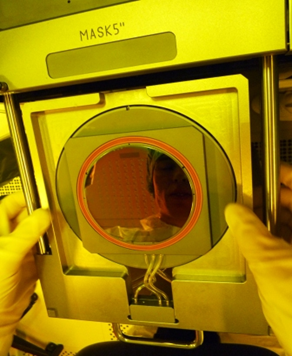
\includegraphics[width=0.9\textwidth, height=5.5cm]{bilder/Maskenjustierer.png}
  \caption{Maskenhalter}
  \label{fig:Maskenjustierer}
\end{minipage}
%\hfill
\begin{minipage}[hbt]{6cm}
    \centering
    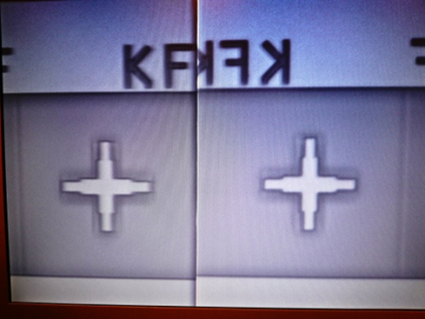
\includegraphics[width=0.9\textwidth,height=4cm]{bilder/Justiervorgang.png}
  \caption{Justiervorgang}
  \label{fig:Justiervorgang}
\end{minipage}

\end{figure}

Der Wafer wurde ausgerichtet, mit dem Vakuum festgehalten und hineingeschoben. Dann justiert man den Wafer so, dass er genau unter der Maske liegt.

Danach drückt man die Taste Exposition und der Wafer wird durch die Maske
belichtet (Abb.\ref{fig:DerMomentderBelichtung } ). Das Licht befindet sich im UV-Bereich.  Bei dem Belichtungsprogramm gibt es verschiedene Belichtungsarten, wir haben uns für die Soft-Kontakt-Belichtungsart entschieden, weil es die schonendste Methode ist. Der Wafer 02 wurde vier Sekunden lang
belichtet. Der Moment der Belichtung ist in der Abbildung \ref{fig:Belichtungsvorgang} zu sehen.


\begin{figure}[H]
\centering
\begin{minipage}[hbt]{6cm}
    \centering
    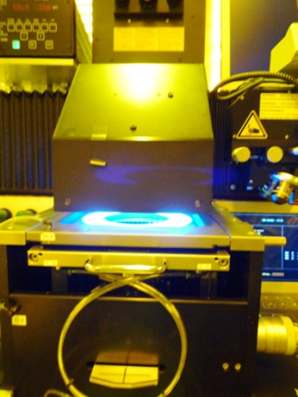
\includegraphics[width=0.8\textwidth, height=6cm]{bilder/Belichtungsvorgang.png}
  \caption{Belichtungsvorgang}
  \label{fig:Belichtungsvorgang}
\end{minipage}
%\hfill
\begin{minipage}[hbt]{6cm}
    \centering
    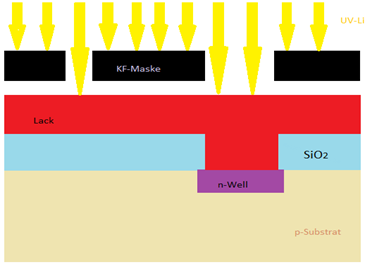
\includegraphics[width=1\textwidth,height=6cm]{bilder/DerMomentderBelichtung.png}
  \caption{ Belichtungsstruktur }
  \label{fig:DerMomentderBelichtung }
\end{minipage}

\end{figure}


Die durchsichtigen Bereiche der Maske lassen das Licht durch und der Wafer wird belichtet.
Durch das Belichten wird der Lack härter. An den Stellen, die nicht belichtet wurden,
wird der Lack später mit einer Rohm-Haas Lösung abgezogen.
Die Belichtungszeit stimmte für den Wafer02, deswegen wurde der Wafer03 auch mit dieser Zeit belichtet. Leider wurde beim Justieren der Wafer03 ein Stückchen Lack an der Maske angeklebt. Wir haben sofort überlegt, ob es beim Entwickeln zu den Fehlern kommen kann.



\paragraph[Entwickeln und Hardbake ]{Entwickeln und Hardbake }

Nach dem Belichtungsprozess wurde der Lack möglichst schnell mit Hilfe von Entwickler Rohm-Haas \ref{fig:Entwickeln} entfernt.
\begin{figure}[H]
\begin{minipage}[hbt]{10cm}
Die Wafer wurden 60 Sekunden lang in dieser Lösung gespült.
Nach dem Entwicklungsprozess muss der Entwickler ganz schnell weg von der Waferoberfläche und sehr gründlich mit dem Wasser abgespült werden (s. Abb. \ref{fig:strukturnachdementwickeln}).
Um den restlichen Lack gegen Ätzmittel noch resistenter zu machen: Hardbake fünf Minuten lang, 120°C .

\end{minipage}
%\hfill
\begin{minipage}[hbt]{4.5cm}
    \centering
    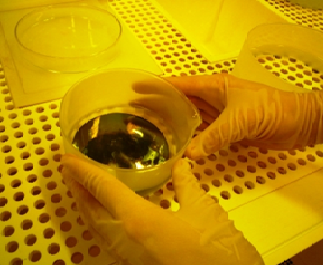
\includegraphics[width=1\textwidth,height=3cm]{bilder/Entwickeln.png}
  \caption{Entwickeln}
  \label{fig:Entwickeln}
\end{minipage}

\end{figure}

\begin{figure}[H]
    \centering
        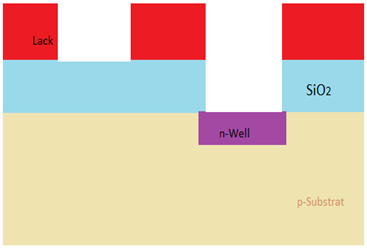
\includegraphics[width=0.5\textwidth]{bilder/StrukturnachdemEntwickeln.png}
    \caption{Struktur nach dem Entwickeln}
    \label{fig:strukturnachdementwickeln}
\end{figure}

\subsubsection[Sichtkontrolle]{Sichtkontrolle}

\paragraph[Mit dem Lichtmikroskop]{Mit dem Lichtmikroskop:}

Nun sollen die Wafer mit dem Mikroskop untersucht werden.
Wie wir es schon erwartet haben, der angeklebte Lack hat sich bemerkbar gemacht: Die Struktur ist nicht mehr sehr deutlich zu sehen, viele untergeätzte Stellen (Abb. \ref{fig:Mikroskopbild3}):

%\hfill
\begin{figure}[H]
    \centering
    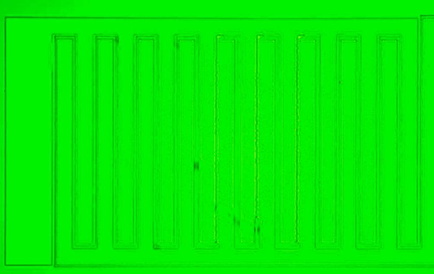
\includegraphics[width=0.5\textwidth]{bilder/Mikroskopbild3.png}
  \caption{Lichtmikroskopbild}
  \label{fig:Mikroskopbild3}
\end{figure}


\paragraph[Dektak-Messung]{Dektak-Messung:}

Nun wurden die Lackdicken von den Wafern 02 und 03 am Dektak gemessen.
Der Dektak ist ein Profilometer mit dem sich die mikroskopische Oberflächenrauigkeit ermitteln lässt.
Ein Mal haben wir über dem p- und das andere Mal über dem n-Pad gemessen \ref{fig:MessungenamDektak}:


\begin{figure}[H]
    \centering
        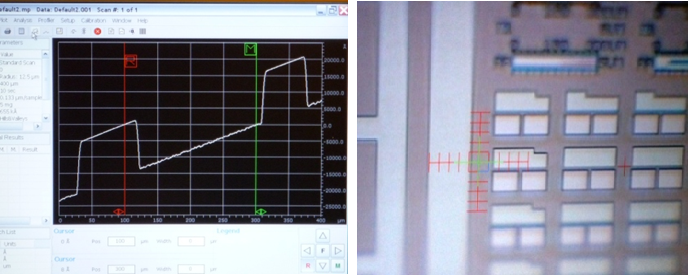
\includegraphics[width=0.75\textwidth]{bilder/MessungenamDektak.png}
    \caption{Messungen am Dektak}
    \label{fig:MessungenamDektak}
\end{figure}


Die Tabelle \ref{tab:Messergebnisse der Lackdickenmessung} zeigt das Ergebnis:

\begin{table}[htbp]
\centering
\caption{Messergebnisse der Lackdickenmessung}
\begin{tabular}{|c|c|c|}

       \hline
       Wafer  & p-Pad & n-Pad \\
        \hline
       120502      & 1.5 $\mu$m & 185 nm       \\
        \hline
       120503    & 1.55 $\mu$m  & 182 nm        \\
        \hline

\end{tabular}
\label{tab:Messergebnisse der Lackdickenmessung}
\end{table}


\paragraph[Ätzen]{Ätzen}

Diesmal wurde das Ätzen vorsichtig mehrmals durchgeführt. Dafür haben wir 1\%-ige gepuffte Flusssäure BHF (HF/$NH_3F$) benutzt. Jeder Wafer wurde in dieser Lösung für ca. eine min. eingetaucht und sofort mit Di-Wasser abgespült. So entstehen die Oxidfenster (Abb. \ref{fig:StrukturnachdemAetzen2}).


\begin{figure}[H]
    \centering
        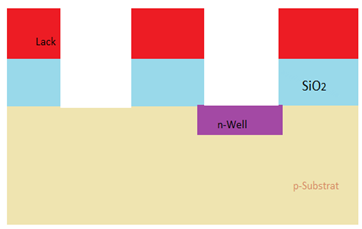
\includegraphics[width=0.5\textwidth]{bilder/StrukturnachdemAetzen2.png}
    \caption{Struktur nach dem Ätzen}
    \label{fig:StrukturnachdemAetzen2}
\end{figure}

Zwischen den Ätzungen haben wir ständig die Oxiddicke mit Dektak kontrolliert. Die Dektakmessung zeigte uns, dass der Ätzvorgang sehr langsam abläuft. Die Kontrolle am Lichtmikroskop hat aber folgendes gezeigt \ref{fig:LichtmikroskopbilderW23}:
Wafer03 wurde total übergeätzt! Starke Dotierung wurde als mögliche Ursache dafür vermutet.

\begin{figure}[H]
    \centering
        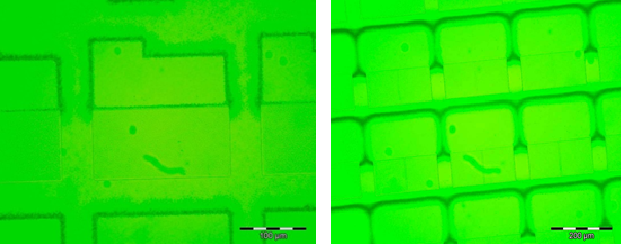
\includegraphics[width=0.7\textwidth]{bilder/LichtmikroskopbilderW23.png}
    \caption{Lichtmikroskopbilder, Wafer 02 und 03}
    \label{fig:LichtmikroskopbilderW23}
\end{figure}


Da der Wafer03 übergeätzt wurde, haben wir entschieden, dass es keine AL-Metallisierung bei ihm durchgeführt wird.
Dagegen Wafer02 war in Ordnung, nur die Kanten waren unscharf(s. Abb. \ref{fig:LichtmikroskopbilderW23}).


\paragraph[Lack entfernen]{Lack entfernen}

Als letztes wurde der Lack von den Wafern 02 und 03 mit dem Aceton entfernt.
Nach dem Lithographie-Schritt sieht unsere Struktur folgendermaßen aus (Abb. \ref{fig:KontaktfenstergeaetztundLackentfernt}):


\begin{figure}[H]
    \centering
        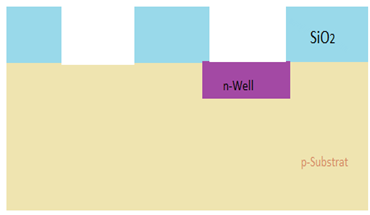
\includegraphics[width=0.5\textwidth]{bilder/KontaktfenstergeaetztundLackentfernt.png}
    \caption{Kontaktfenster geätzt und Lack entfernt}
    \label{fig:KontaktfenstergeaetztundLackentfernt}
\end{figure}

Anschließend wurden von allen drei Wafer die organische Stoffe mit dem Ätzmittel Caro's Etch entfernt.




\subsection[Tag 3]{Tag 3}

\subsubsection[PVD \& Metallisieren ]{PVD \& Metallisieren : }

 PVD (physical vapour deposition) ist die physikalische Gasphasenabscheidung, die für die vakuumbasierten  Beschichtung mit Aluminium verwendet wird.
\begin{figure}[H]
\begin{minipage}[hbt]{9cm}

Die Abbildung \ref{fig:SchematischeDarstellungeinesPVD-Verdampfungsverfahrens} zeigt die schematische Darstellung eines PVD-Verdampfungsverfahrens.

Das abzuscheidende Material (Target) liegt in fester Form vor. Mit dem Laser- oder Elektronenstrahl, der von einer Elektronenquelle geschossen werden, werden die Ionen oder Elektronen durch ein elektromagnetisches System auf das Target umgelenkt und das Material wird verdampft.

Das  Material verdampft  wegen des sehr niedrigen Druckes und der Energie der Elektronen. Es bildet sich ein Dampf, der durch elektrische Felder durch die Kammer geführt wird. Dabei trifft  der Dampf auf die zu beschichtenden Teile und es kommt zu einer Schichtbildung.
Die Elektronenstrahlkanonen setzen ein Vakuum voraus, deswegen wurde das Vakuum in der Bedampfungsanlage (s. Abb. \ref{fig:Bedampfungsanlage}) über die Nacht abgepumpt.

\end{minipage}
%\hfill
\begin{minipage}[hbt]{6cm}
    \centering
    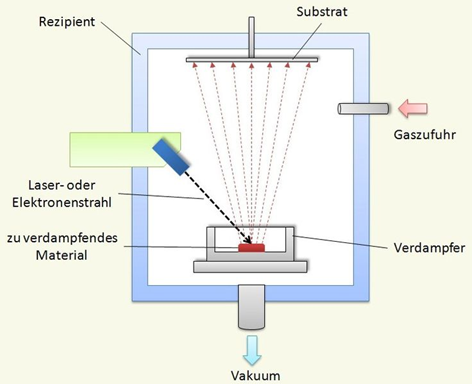
\includegraphics[width=1\textwidth,height=7cm]{bilder/SchematischeDarstellungeinesPVD-Verdampfungsverfahrens.png}
  \caption{PVD-Verfahren}
  \label{fig:SchematischeDarstellungeinesPVD-Verdampfungsverfahrens}
\end{minipage}

\end{figure}

\begin{figure}[H]
    \centering
        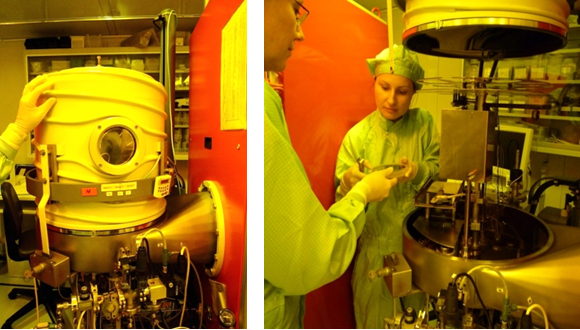
\includegraphics[width=0.6\textwidth]{bilder/Bedampfungsanlage.png}
    \caption{Bedampfungsanlage}
    \label{fig:Bedampfungsanlage}
\end{figure}


Bevor der Wafer in die PVD-Anlage platziert wird, wurde die Waferoberfläche noch Mal mit einer  1\%-igen HF-Lösung (HF-Dip) für 15 Sekunden gereinigt. Diese Lösung dient dazu, die neuentstandene Oxidschicht zu entfernen.
Danach wurde unser einziger Wafer02 in den PVD-Apparat mit der Vorderseite nach unten eingelegt. Außer des Einlegens des Wafers wurden alle Schritte mit Hilfe der Steuerungstasten automatisch ausgeführt.
Dann wird das Programm eingestellt und der PVD-Prozess fängt an. Die aufzusputternde AL-Schicht soll 500 nm betragen.

Da der PVD-Prozess 30 Minuten dauerte, wurden inzwischen Wafer 01 und 03 noch Mal mit Phosphorus beschichtet. Anschießend wurden die Wafer 30 Minuten lang mit 200°C gebacken. Diese Improvisation war notwendig, da die beiden Wafer keine Oxidschicht mehr hatten.
Nach PVD wurde Wafer02 mit einer Salpetersäure zehn Minuten lang behandelt.
Anschießend backte  der Wafer 30 Minuten lang bei einer Temperatur von 140°C(da Al Kristalline bei 200°C bildet).

\begin{figure}[H]
    \centering
        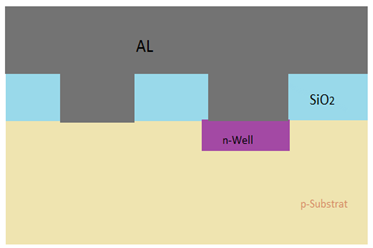
\includegraphics[width=0.5\textwidth]{bilder/Wafer02NachderMetallisierung.png}
    \caption{Wafer02 nach der Metallisierung}
    \label{fig:Wafer02NachderMetallisierung}
\end{figure}

\paragraph[Wafer für den Schrägschliff brechen]{Wafer für den Schrägschliff brechen }


Weiter wurden Wafer 01 und 03 für den Schrägschliffwinkel gebrochen.
Die Wafer wurden zuerst in der Mitte angeritzt. Unter den Wafer an dieser angeritzten
Stelle haben wir eine alte Probe gelegt und dann durch einen leichten Druck den Wafer
zum Brechen gebracht .Es ist leicht durchzuführen, da Silizium entlang der
Kristallrichtung bricht. Die entstandenen Proben haben die Abmessungen ca. 5x5 $mm^{2}$.
Die Proben wurden in den vormarkierten Kästchen gelegt.



\subsubsection[Lithographie mit der AL-Maske]{Lithographie mit der AL-Maske }

Nun werden die typischen Lithographie-Schritte bei leicht abgeänderten Bedingungen noch Mal durchgeführt.

\paragraph[Prebake, Belacken, Softbake]{Prebake, Belacken, Softbake}


Die Flüssigkeitsreste werden entfernt, indem die Wafer 30 min. lang bei 140°C auf der Heizplatte liegen bleiben.

Danach wird der Wafer 02 mit einem Lack  Az 52/4 beschichtet und anschließend zwei Minuten lang bei 95°C getrocknet. Die Ruhezeit beträgt eine Stunde.


\paragraph[Belichten mit Al-Maske]{Belichten mit Al-Maske  }


Der Wafer02 wird genau so belichtet, wie oben schon beschrieben wurde ( s. Lithographie am Tag2),(s. Abb. \ref{fig:BelichtendurchMEMaske}) Bemerkung: Die Al-Maske wurde auch nach AA-Maske justiert, und die Belichtungszeit beträgt jetzt nur 3,7 Sekunden, da Aluminium glänzend ist und Licht reflektiert.

 Danach wurde der Lack mit der Rohm Haas-Lösung entwickelt (Abb. \ref{fig:NachdemEntwickeln}).


\begin{figure}[H]
\centering
\begin{minipage}[hbt]{6cm}
    \centering
    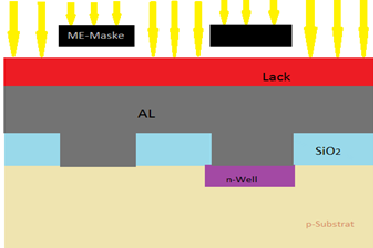
\includegraphics[width=1\textwidth, height=4.5cm]{bilder/BelichtendurchMEMaske.png}
  \caption{Belichten durch die ME-Maske}
  \label{fig:BelichtendurchMEMaske}
\end{minipage}
\hfill
\begin{minipage}[hbt]{7cm}
    \centering
    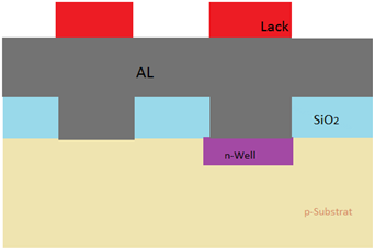
\includegraphics[width=1\textwidth,height=4.5cm]{bilder/NachdemEntwickeln.png}
  \caption{Struktur nach dem Entwickeln }
  \label{fig:NachdemEntwickeln}
\end{minipage}

\end{figure}


\paragraph[Sichtkontrolle]{Sichtkontrolle}

Nun soll der Wafer mit dem Lichtmikroskop untersucht werden. Wenn der Lack nicht bis zum Ende entwickelt wurde, kann man die Lichtinterferenz sehen, was wir auch in den kleinen Mengen gesehen haben.

Dektak-Messung ergab, dass die Dicke nur 1,36 $\mu$m ist, aber wir brauchen mindestens 1,5 $\mu$m. Deswegen wurde entschieden, noch Mal zehn Sekunden lang Nachentwicklung zu machen. Nächste Messung ergab 1,35 $\mu$m. Danach wurde der Wafer noch mit dem Photometer untersucht und es sprach nichts dagegen, dass der Lack nicht entwickelt wurde.



\paragraph[Ätzen]{Ätzen}

\vspace{10mm}
Vor dem Ätzen wird der Wafer noch für fünf Minuten lang auf die Heizplatte bei 140°C gelegt.
Der Ätzvorgang wird diesmal mit einer Ätzmischung aus der Phosphorsäure, Essigsäure, Wasser und der Salpetersäure durchgeführt($H_{3}PO_{4}$ +$H_{2}O$+$HNO_{3}$). Es wurde mehrmals in der Zehner-Intervall (je zehn Sekunden in der Lösung) geätzt, danach wurde schnell in das Di-Wasser eingetaucht und abgespült.  Nach der Sicht wurde beurteilt, ob die Al-Schicht weggeätzt wurde(Abb. \ref{fig:AlSchichtaetzen}). Beobachtung: viel Bläschen.

\begin{figure}[H]
    \centering
        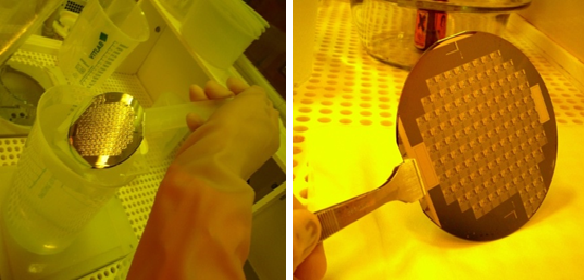
\includegraphics[width=0.7\textwidth]{bilder/AlSchichtaetzen.png}
    \caption{Al-Schicht ätzen}
    \label{fig:AlSchichtaetzen}
\end{figure}


\begin{figure}[H]
    \centering
        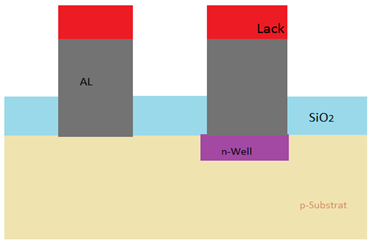
\includegraphics[width=0.6\textwidth]{bilder/StrukturnachdemAetzvorgang.png}
    \caption{Struktur nach dem Ätzvorgang}
    \label{fig:StrukturnachdemAetzvorgang}
\end{figure}


\paragraph[Kontrolle mit dem Lichtmikroskop]{Kontrolle mit dem Lichtmikroskop }


Die Untersuchung mit dem Lichtmikroskop hat uns gute Bilder geliefert: Die Kontakte sehen gut aus, nur ein wenig untergeätzt (dunkler Rand, s. Abb. \ref{fig:Lichtmikroskopbilder4}).


\begin{figure}[H]
    \centering
        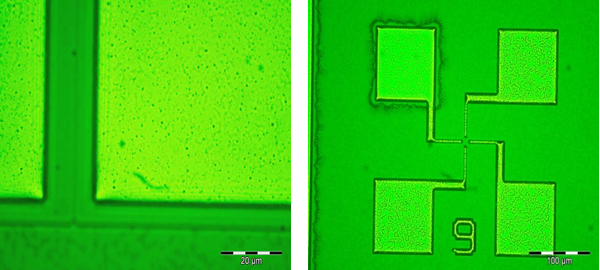
\includegraphics[width=0.6\textwidth]{bilder/Lichtmikroskopbilder4.png}
    \caption{Lichtmikroskopbilder}
    \label{fig:Lichtmikroskopbilder4}
\end{figure}

\paragraph[Photolack entfernen]{Photolack entfernen}


Als letzter Schritt wird der Lack entfernt. Diesmal wird er in das Aceton für drei Minuten eingetaucht, danach sehr schnell mit Wasser gesäubert. Anschließend wurde unser Wafer
in einem Ultraschalbad gereinigt(Abb. \ref{fig:Ultraschalbad}).

\begin{figure}[H]
\centering
\begin{minipage}[hbt]{5cm}
    \centering
    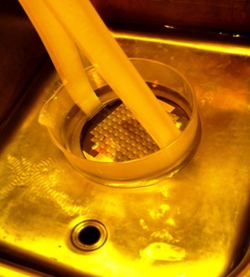
\includegraphics[width=1\textwidth, height=4cm]{bilder/Ultraschalbad.png}
  \caption{Ultraschalbad}
  \label{fig:Ultraschalbad}
\end{minipage}
\hfill
\begin{minipage}[hbt]{8cm}
    \centering
    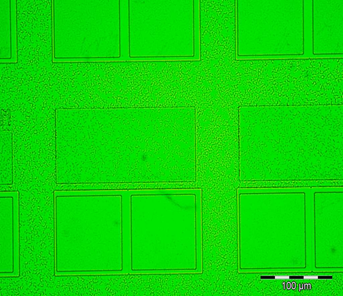
\includegraphics[width=0.9\textwidth,height=4cm]{bilder/LichtmikroskopbildEndstruktur.png}
  \caption{Lichtmikroskopbild:Endstruktur}
  \label{fig:LichtmikroskopbildEndstruktur}
\end{minipage}

\end{figure}


Am Ende haben wir unseren Wafer noch Mal am Lichtmikroskop untersucht. Die Ergebnisse waren gut: Kanten sind sehr glatt, sehr gute, klare Struktur (s. Abb. \ref{fig:LichtmikroskopbildEndstruktur}).


\paragraph[Enddickenmessung]{Enddickenmessung}

Die Aluminiumdickenmessung mit dem Profilometer ergab die Werte zwischen 470 nm und 490 nm, was dem theoretisch erwarteten Wert von 500 nm entsprach.

\paragraph[Tempern ]{Tempern}

Dieser Temperaturprozess dient der Verbesserung der Kontakte  zwischen dem Aluminium und dem Substrat. Dafür wurde der Wafer bei 400°C für 30 Minuten im Ofen erhitzt.


\subsubsection[Endergebnis]{Endergebnis}
Unser Endergebnis, also ein pn-Übergang, ist schematisch  in der Abbildung \ref{fig:Endstruktur} dargestellt.

\begin{figure}[H]
    \centering
        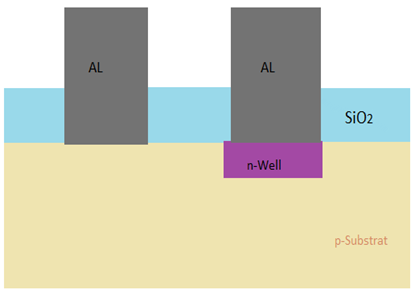
\includegraphics[width=0.5\textwidth]{bilder/Endstruktur.png}
    \caption{Endstruktur}
    \label{fig:Endstruktur}
\end{figure}

Endergebnis: Wafer 120502

\begin{figure}[H]
    \centering
        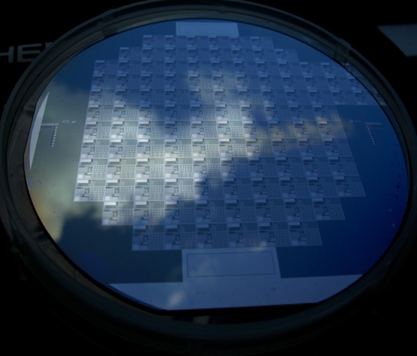
\includegraphics[width=0.6\textwidth]{bilder/EndergebnisWafer120502.png}
    \caption{Endergebnis: Wafer 120502}
    \label{fig:EndergebnisWafer120502}
\end{figure}



\subsection[Tag 4]{Tag 4}

\subsubsection[Schrägschliff]{Schrägschliff }

Um die pn-Übergangstiefe zu messen wurden unsere Proben zuerst geschliffen (weil die pn-Tiefe nicht direkt mit dem Mikroskop gemessen werden kann).
Jede Probe wird zuerst auf einen Support geklebt, indem man den Support auf einer Heizplatte bei 120°C heizt und der spezielle Klebstoff darauf geschmolzen wird (s.Abb. \ref{fig:KlebstoffunddieProben} und \ref{fig:ZubereitungzumSchleifen} ).

\begin{figure}[H]
\centering
\begin{minipage}[hbt]{6cm}
    \centering
    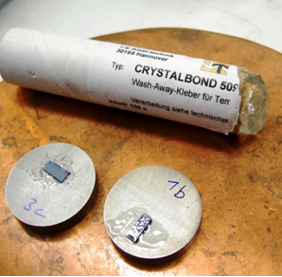
\includegraphics[width=0.8\textwidth, height=4.5cm]{bilder/KlebstoffunddieProben.png}
  \caption{Klebstoff mit Proben}
  \label{fig:KlebstoffunddieProben}
\end{minipage}
\hfill
\begin{minipage}[hbt]{7cm}
    \centering
    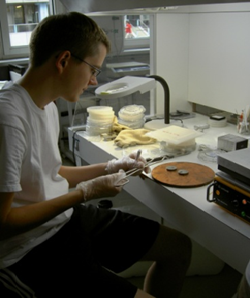
\includegraphics[width=1\textwidth,height=6cm]{bilder/ZubereitungzumSchleifen.png}
  \caption{Zubereitung zum Schleifen}
  \label{fig:ZubereitungzumSchleifen}
\end{minipage}

\end{figure}



Die Proben werden dann mit einem Schleifmittel (Suspension DP aus Diamantpartikeln) fünf Minuten lang geschliffen(s. Abb. \ref{fig:Schleifen} ), so dass sie am Rand einen Schrägschliff (s.Abb. \ref{fig:SchraegschliffunterdemMikroskop}) bekommen. Danach werden die Proben abgespült und getrocknet.

\begin{figure}[H]
\centering
\begin{minipage}[hbt]{6cm}
    \centering
    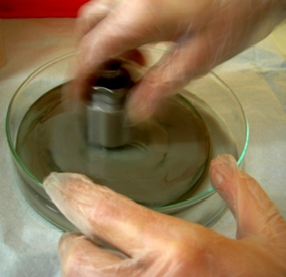
\includegraphics[width=0.8\textwidth, height=4cm]{bilder/Schleifen.png}
  \caption{Schleifen}
  \label{fig:Schleifen}
\end{minipage}
\hfill
\begin{minipage}[hbt]{7cm}
    \centering
    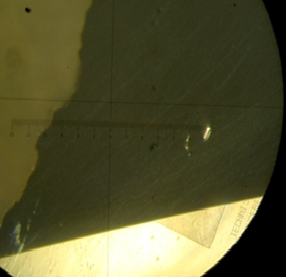
\includegraphics[width=0.8\textwidth,height=4cm]{bilder/SchraegschliffunterdemMikroskop.png}
  \caption{Schrägschliff }
  \label{fig:SchraegschliffunterdemMikroskop}
\end{minipage}

\end{figure}


\subsubsection[Dekoration]{Dekoration }


Zuerst wurde mit der $HF:CH_{3}COOH:HNO_{3}$ (1:4:5) Lösung versucht, die Probe zu dekorieren. Es hat nicht funktioniert und deswegen wurde entschlossen, mit der Verkupferung zu versuchen.

Die Dekoration der Proben wird dann im Reinraum mit einer Lösung aus zwei Gramm
$CuSO_{4}$, fünf ml HF(40\%) und 100 ml $H_{2}O$ dekoriert. Am Anfang des Vorgangs liegen die
Proben in der Lösung mit der Vorderseite nach oben(Abb. \ref{fig:Verkupferung}). Sie werden dann mit zwei ''Schwanenhals''-Lampen drei bis fünf Sekunden belichtet, damit das Licht den Prozess aktivieren kann (Abb. \ref{fig:Schwanenhalslampen}).

\begin{figure}[H]
\centering
\begin{minipage}[hbt]{6cm}
    \centering
    \includegraphics[width=0.8\textwidth, height=4cm]{bilder/Verkupferung.png}
  \caption{Verkupferung}
  \label{fig:Verkupferung}
\end{minipage}
\hfill
\begin{minipage}[hbt]{7cm}
    \centering
    \includegraphics[width=0.8\textwidth,height=4cm]{bilder/Schwanenhalslampen.png}
  \caption{Schwanenhalslampen}
  \label{fig:Schwanenhalslampen}
\end{minipage}

\end{figure}



Die Kupferlösung wird auf der Oberfläche der Probe an dem angeschliffenen Gebiet aufgetragen. Da die Kupfermischung einen Mangel an den Elektronen hat, lagert sich diese Lösung an dem n-Gebiet, wo es mehr Elektronen gibt. Deswegen erscheint die n-leitende Seite des pn-Übergangs heller getönt als die p-leitende Seite (s.Abb. \ref{fig:DekorationunterdemLichtmikroskop}). Anschließend werden die Proben mit dem Aceton gereinigt.

\begin{figure}[H]
\centering
\begin{minipage}[hbt]{6cm}
    \centering
    \includegraphics[width=1\textwidth, height=5cm]{bilder/DekorationunterdemLichtmikroskop.png}
  \caption{Dekoration unter dem Lichtmikroskop}
  \label{fig:DekorationunterdemLichtmikroskop}
\end{minipage}
\hfill
\begin{minipage}[hbt]{7cm}
    \centering
    \includegraphics[width=1\textwidth,height=5cm]{bilder/pn-TiefemessungmitdemDektak.png}
  \caption{pn-Tiefemessung mit dem Dektak}
  \label{fig:pn-TiefemessungmitdemDektak}
\end{minipage}

\end{figure}

\subsubsection[Auswertung der Junction Tiefe ]{Auswertung der Junction Tiefe}

Unter dem Mikroskop ist dieser Unterschied gut sichtbar und lässt sich ohne Schwierigkeiten auswerten(es wird die Länge der Verkupferung l gemessen, s.Abb. \ref{fig:SchematischeDarstellungzumAusrechnenderpnTiefe}):

\vspace{3mm}
\begin{center}
Wafer01\_a: 80 $\mu$m

Wafer01\_b: 75 $\mu$m
\end{center}

Dektak-Messung:
\vspace{1mm}

    \hspace{15mm}       Wafer01\_b:
\vspace{1mm}
\begin{center}

Tiefe 7,0 $\mu$m, Länge 300 $\mu$m

Tiefe 6,9 $\mu$m, Länge 300 $\mu$m
\end{center}

    \hspace{15mm}        Wafer01\_a:

\vspace{1mm}
\begin{center}

    Tiefe 6,2 $\mu$m, Länge 300 $\mu$m

    Tiefe 5,7 $\mu$m, Länge 300 $\mu$m

\end{center}

Daraus kann man die Junctions-Tiefe ausrechnen:

\begin{figure}[htbp]
    \centering
        \includegraphics[width=0.5\textwidth]{bilder/SchematischeDarstellungzumAusrechnenderpnTiefe.png}
    \caption{Schematische Darstellung zum Ausrechnen der pn-Tiefe}
    \label{fig:SchematischeDarstellungzumAusrechnenderpnTiefe}
\end{figure}

Nach  der Beziehung $x_j$=sin $\alpha$, haben wir folgende Ergebnisse ausgerechnet:

\vspace{3mm}
    \hspace{15mm} Wafer01\_b:

\begin{center}
    1,52 $\mu$m und 1,65 $\mu$m
\end{center}

    \hspace{15mm}   Wafer01\_a:

\begin{center}
    1,76 $\mu$m und 1,70 $\mu$m
\end{center}

Die ausgerechneten Werte entsprechen unseren Erwartungen, was ein Indiz dafür ist, dass die Prozessschritte richtig gemacht wurden.

So endet unser Praktikum im Reinraum.



\subsection[Schlussbetrachtung]{Schlussbetrachtung}

Als Ergebnis unserer Tätigkeit haben wir nur einen Wafer mit vielen pn-Übergängen angefertigt. Die anderen Wafer haben wir für den Schrägschliff verwendet.

Insgesamt haben alle Teilnehmer durch diese vier Tage im Reinraumlabor viel Wissen über die Arbeit im Reinraum, den Umgang mit gefährlichen Stoffen, Arbeit am Mikroskop und Profilometer, und die Herstellungsprozesse eines pn-Übergangs erworben.
Praktische Arbeit hat unser theoretisches Wissen sehr bereichert.


\begin{figure}[H]
    \centering
        \includegraphics[width=1\textwidth]{bilder/Endbild.png}
    \caption{Laborteilnehmer und Betreuer in Reinraumkleidung}
    \label{fig:Endbild}
\end{figure}


%--------------------------------------------------------------------
%--------------------------------------------------------------------

\newpage

\section{Kennlinie}
\begin{quote}
    \subsection{Messaufbau}
    \begin{quote}
        Die erste Untersuchung, der wir unsere Dioden unterzogen haben, war die Aufnahme der Kennlinien. Dazu muss der
        pn-Übergang unter einem Lichtmikroskop kontaktiert werden. Die beiden Gebiete werden jeweils mit einem Kanal des
        Parameter-Analyzer 4145A von HP verbunden, der einen sweep der Spannung von \SI{-1}{\volt} bis \SI{1}{\volt} macht
        und dabei den Strom misst.\\
        Diese Messung haben wir auf verschiedenen Dies durchgeführt um diese miteinander vergleichen zu können.

    \end{quote} % Sub: Messaufbau


    \subsection{Auswahl der zu messenden Diode}
    \begin{quote}
        Um möglichst aussagekräftige Messwerte zu erhalten, haben wir uns dazu entschieden jeweils die größte Diode auf
        den Dies für unsere Messungen zu benutzen. Davon haben wir uns versprochen, dass sowohl Durchlass- als
        auch Sperrstrom am größten sind und somit besser zu messen sein würden als bei kleineren Dioden.
        Nach der Auswertung anderer Messungen und einigen weiteren Überlegungen stellte sich jedoch heraus, dass
        dies ein Trugschluss war. Eine größere, quadratische Diode führt zwar sehr wohl einen höheren Strom als eine
        kleinere quadratische. Bei Durchlass- und Sperrstrom kommt es aber nicht auf die Größe sondern auf die
        Fläche des pn-Übergangs an. Daher kann eine der Fläche nach nur halb so große Diode, mit verzahnter
        Fingerstruktur, mehr Strom führen als die flächenmäßig größte Diode, für die wir uns entschieden haben. Deshalb
        wird am Ende der Auswertung zusätzlich noch eine solche Fingerstruktur betrachtet.

    \end{quote} % Subsub: Auswahl der zu messneden Diode


    \subsection{Erwartete Kennlinie}
    \begin{quote}

        \subsubsection{Dunkelkennlinie}
        \begin{quote}



            Bei intakten Dioden erwarten wir im Grunde eine Kennlinie nach der Formel von Shockley (Gl. \ref{equ:Schockley})
            jedoch inklusive realitätsbedingter Abweichungen.



            \begin{equation}
            \begin{split}
            J_{ges} = J_0 \cdot (e^ \frac{U}{U_t} -1)
            \end{split}
            \label{equ:Schockley}
            \end{equation}




            \begin{figure}[htbH]
                \centering
                \includegraphics[scale=0.7, trim = 0cm 0cm 0cm 0cm, clip]{KennlinienBilder/reale_Kennlinie}
                \caption{Reale kennlinie einer Diode}
                    \begin{center}
                        \vspace{0.5em}
                        \small Quelle: Laborskript Technologie und Bauelemente der Halbleitertechnik (Aydin Asri,
                                        Arminius Kuckelt, Michael Sadowski, Julian Utehs und Tristan Visentin) S.66
                    \end{center}
                \label{fig:reale_Kennlinie}
            \end{figure}

\vspace{2.5em}
            Wie in Abb. \ref{fig:reale_Kennlinie} logatythmisch dargestellt erwarten wir, dass nur der mittlere Teil
            zwischen \SI{0,2}{\volt} und \SI{0,5}{\volt} der Schockley-Gleichung folgt. Bei höheren Spannungen ist der
            Wiederstand der Bahngebiete nicht mehr vernachläs\-sigbar klein und wirkt sich deutlich strommindernd auf
            die Kennlinie aus. Außerdem wird sich durch die Nichteinhaltung der Shockleybedingungen die
            Rekombination in der Raumladungszone bemerkbar machen. Bei kleinen Spannungen (unter ca.
            \SI{0,2}{\volt}) fließt deutlich mehr Strom aufgrund von Rekombination als durch den Potentialunterschied,
            wodurch der mehr Strom fließt als nach Gl. \ref{equ:Schockley}.\\

            Die in Abb. \ref{fig:reale_Kennlinie} dargestellte mangelhafte Messgenauigkeit haben wir nicht erwartet. Wir
            sind davon ausgegangen, dass selbst bei sehr guten Dioden, also in diesem Fall welchen mit sehr kleinen
            Sperrströmen, der Parameter-Analyzer keine Probleme hat diese zu messen.\\
            \\
            Wir werden den Strom betragsmäßig über der Spannung auftragen, was es ermöglicht, zur illustration auch
            negative Ströme logarythmisch dar zu stellen. In unserer Auswertung sind Ströme bei negativen Spannungen
            also als negative Ströme auf zu fassen.

        \end{quote} % Subsub: Dunkelkennlinie


        \subsubsection{Beleuchtete Kennlinie}
        \begin{quote}

            Unter Lichteinfluss ist die theoretische Kennlinie einer Diode wie folgt:

            \begin{equation}
            \begin{split}
            J_{ges} &= J_0 \cdot (e^ \frac{U}{U_t} -1) - J_{ph}\\
            J_{ph} &= g \p e \p (L_n + L_p)
            \end{split}
            \label{equ:Schockley_photo}
            \end{equation}

            Wir erwarten also insgesamt kleinere Durchlassströme und damit eine größere Druchlassspannung. Außerdem
            müsste der Sperrstrom durch die zusätzliche Generation größer werden.

        \end{quote} % Subsub: Beleuchtete Kennlinie





    \end{quote} % Sub: Erwartete Kennlinie


    \subsection{Messergebnisse}
    \begin{quote}

        \subsubsection{Dunkelkennlinie}
        \begin{quote}

            Die ersten Messungen haben wir mit folgendem Ergebniss unter Einfluss des Raumlichtes durchgeführt:

            \begin{figure}[H]
                \centering
                \includegraphics[scale=0.7, trim = 3.1cm 9.2cm 4cm 8.5cm, clip]{KennlinienBilder/raumlicht_kennlinie}
                \caption{Diodenkennlinie unter Raumlichteinfluss}
                \label{fig:raumlicht_kennlinie}
            \end{figure}

            Wie in Abb. \ref{fig:raumlicht_kennlinie} gut zu erkennen, ist der Einfluss des Raumlichtes groß genug um die
            Durchlassspannung auf fast \SI{0,3}{\volt} zu heben. Da das Raumlicht sich offensichtlich so gravierend auf
            die Kennlinie auswirkt haben wir den Messaufbau für alle folgenden Messungen abgedunkelt.
            Außerdem war die Strombegrenzung zu gering eingestellt. Auch das ist in den weiteren Messungen korrigiert.
            \\
            Die folgenden Messungen stammen aus der mittleren Spalte Dies ganz oben, in der Mitte und ganz unten.


            \begin{figure}[H]
                \centering
                \includegraphics[scale=0.7, trim = 3.1cm 9.2cm 4cm 8.5cm, clip]{KennlinienBilder/dunkel_kennlinie_z1_s6.pdf}
                \caption{Dunkelkennlinie der großen Diode auf dem Die z1s6}
                \label{fig:dunkel_kennlinie_z1_s6.pdf}
            \end{figure}


            \begin{figure}[H]
                \centering
                \includegraphics[scale=0.7, trim = 3.1cm 9.2cm 4cm 8.5cm, clip]{KennlinienBilder/dunkel_kennlinie_z6_s6.pdf}
                \caption{Dunkelkennlinie der großen Diode auf dem Die z6s6}
                \label{fig:dunkel_kennlinie_z6_s6.pdf}
            \end{figure}


            \begin{figure}[H]
                \centering
                \includegraphics[scale=0.7, trim = 3.1cm 9.2cm 4cm 8.5cm, clip]{KennlinienBilder/dunkel_kennlinie_z12_s6.pdf}
                \caption{Dunkelkennlinie der großen Diode auf dem Die z12s6}
                \label{fig:dunkel_kennlinie_z12_s6.pdf}
            \end{figure}


            Zum Vergleich noch die Messung der Fingerstruktur.

            \begin{figure}[H]
                \centering
                \includegraphics[scale=0.7, trim = 3.1cm 9.2cm 4cm 8.5cm, clip]{KennlinienBilder/finger_dunkel_kennlinie_z6_s6.pdf}
                \caption{Dunkelkennlinie der großen Diode mit Fingerstruktur auf dem Die z6s6}
                \label{fig:finger_dunkel_kennlinie_z6_s6.pdf}
            \end{figure}



        \end{quote} % Subsub: Dunkelkennlinie


        \subsubsection{Beleuchtete Kennlinie}
        \begin{quote}
            
            Um die beleuchtete Kennlinie auf zu nehmen haben wir die Lichtquelle des Microskops während der Messung
            einer großen Diode angeschaltet gelassen.
            
            \begin{figure}[H]
                \centering
                \includegraphics[scale=0.7, trim = 3.1cm 9.2cm 4cm 8.5cm, clip]{KennlinienBilder/beleuchtete_kennlinie_z7_s7.pdf}
                \caption{Kennlinie der beleuchteten Diode auf dem Die z6s6}
                \label{fig:beleuchtete_kennlinie_z7_s7.pdf}
            \end{figure}
            
        \end{quote} % Subsub: Beleuchtete Kennlinie
        


    \end{quote} % Sub: Messergebnisse




    \subsection{Auswertung}
    \begin{quote}
        
        Zuerst einmal scheinen fast alle der gemessenen Dioden zu funktionieren, sich also wie erwartet zu verhalten.
        Wir haben die Prozessschritte bei der Herstellung also insofern erfolgreich durchgeführt, als dass auf dem Wafer
        funktionsfähige Dioden entstanden sind.\\
        Entgegen unserer ursprünglichen Vermutung war der Parameter-Analyzer nicht in der Lage die kleinsten Ströme, die
        wir hätten messen wollen, auf zu zeichnen. Dies ist deutlich im linken Teil der Abbildungen
        \ref{fig:dunkel_kennlinie_z1_s6.pdf} und \ref{fig:dunkel_kennlinie_z6_s6.pdf} zu erkennen. Hier konnte unser
        Messgerät die Sperrspannung der Diode nicht mehr aufzeichnen, was jedoch für den von uns hergestellten
        pn-Übergang spricht. Die Sperrspannung beträgt bei den oben genannten Messungen unter \SI{0,1}{\nano\ampere},
        wobei $J_0$ $\approx$ \SI{3}{\pico\ampere} ist und der Durchlassstrom bei ca. \SI{100}{\milli\ampere} liegt.
        \\
        Diese Werte lassen sich nur schwer mit z.B. handelsüblichen Dioden vergleichen, da von den Herstellern keine
        Angaben etwa zu Dotierstoffkonzentration und pn-Übergangsfläche gemacht werden. Bei Sperrströmen unter
        \SI{0,1}{\nano\ampere} kann man aber davon ausgehen, dass sie digital als Null interpretiert werden, da sie
        selbst von dem Parameter-Analyzer nicht mehr als eindeutiger Strom aufgefasst werden.
        Damit könnte man unsere Dioden durchaus in digitalen Schaltungen einsetzen und hätte nur sehr geringe Leckströme.\\
        
        Beim Prozessieren der Diode auf dem Die z12s6 (Abb. \ref{fig:dunkel_kennlinie_z12_s6.pdf}) scheint etwas schief
        gegangen zu sein. Es ist zwar deutlich zu sehen, dass es eine Diodenkennlinie ist, der Sperrstrom von
        \SI{1}{\nano\ampere} ist aber deutlich größer als bei den anderen Dioden.\\
        
        Bei dem Kennlinienplot der Fingerstruktur (Abb. \ref{fig:finger_dunkel_kennlinie_z6_s6.pdf}) ist deutlich zu
        erkennen, dass der Sperrstrom auf über \SI{0,1}{\micro\ampere} gestiegen ist. Auch $J_0$ ist aufgrund der
        größeren pn-Übergangsfläche auf \SI{30}{\pico\ampere} gestiegen.\\
        
        Abschließend verhielt sich auch die beleuchtete Diode exakt wie erwartet. Im Vergleich zur unbeleuchteten Diode
        sind Sperrstrom und Durchlassspannung deutlich größer wobei $J_0$ in der selben Größenordnung bleibt.
        

    \end{quote} % Sub: Auswertung

%
%
%
%     Quellen:
%     kennlinie: Laborskript Technologie und Bauelemente der Halbleitertechnik (Aydin Asri, Arminius Kuckelt, Michael
%     Sadowski, Julian Utehs und Tristan Visentin) S.66
%


%     unterspannung
%     0.0 & 2.4
%     0.5 & 3.8
%     0.8 & 4.5
%     1.0 & 5.0
%     1.3 & 5.5
%     1.8 & 6.7
%     2.5 & 8.2
%     3.0 & 9.2


    \end{quote} %sec Kennlinie
\newpage
%--------------------------------------------------------------------
%--------------------------------------------------------------------


\section{Schaltverhalten}
\begin{quote}

<<<<<<< HEAD
    \subsection{Einführung}

    In diesem Versuch soll das Schaltverhalten bei Strom- und Spannungssprüngen
    untersucht werden. Ein Maß für die Geschwindigkeit mit der die Diode schalten
    kann ist die Minoritätsträgerlebensdauer. Der Schaltvorgang hält an
    , bis die Minoritäten auf- bzw. abgebaut sind. Daher ist es Ziel dieses
    Versuches über zwei unterschiedliche Verfahren diese Ladungsträgerlebensdauer
    zu bestimmen. Dies ist zum einen der Ausschaltvorgang und zum anderen
    die Stromkommutierung.\\
    \\

    \subsection{Theorie}

    Zunächst sollen das ideale und das reale Schaltverhalten gegenüber gestellt
    werden. Das ideale Verhalten charakterisiert sich durch verzögerungs- und
    verlustfreies Schalten. Die zu messenden Dioden zeigen allerdings durch
    Energiespeicher wie die Sperrschicht- und die Diffusionskapazität kein
    ideales Schaltverhalten. \\

    Dabei ist die Charakteristik des Schaltverhaltens davon abhängig, ob es
    sich um ein Spannungs- oder Stromsprung und einen Ein- oder Ausschaltvorgang
    handelt. Um das Verständnis für diese Vorgänge zu verbessern, soll im
    Folgenden näher auf einige Beispiele eingegangen werden.\\

    Bei einem Einschaltstromsprung werden zwei Fälle unterschieden: Die starke
    und die schwache Injektion. Ob starke oder schwache Injektion vorliegt
    richtet sich nach der Ladungsträgeranzahl, die von der einen Seite des
    pn-Überganges als Majoritätsträger auf die andere Seite als Minoritätsträger
    gelangen. Ist die Anzahl der auf der anderen Seite ankommenden (nun
    Minoritäten) in etwa so groß, oder größer wie die Majoritäten spricht man von
    starker Injekion. Andernfalls spricht man von schwacher Injektion.\\
    Wie in Bild \ref{fig:Stromeinschalten} zu erkennen, hat in den beiden
    Fällen der Bahnwiderstand eine unterschiedlichen Einfluss. Nach Shockley ist der
    Bahnspannungsabfall für schwache Injektion zu vernachlässigen. Mit Hilfe der
    Boltzmanfaktoren lässt sich ein logarthmischer Verlauf der Spannung über der
    RLZ herleiten. Dieser ist in der Abbildung \ref{fig:Stromeinschalten} in der
    grob gestrichelten Kennlinie zu erkennen. Man könnte vermuten, dass ohne den
    Bahnwiderstand nur der kapazitive Anteil zur Wirkung kommt und die Spannung
    daher kaum springen darf.\\
    Kommt hingegen der Einfluss des Bahnwiderstandes bei der starken Injektion
    hinzu, dann kann ein heftiger Spannungssprung erfolgen. Der zusammengefasste
    Spannungsverlauf ist in Bild \ref{fig:Stromeinschalten} an der
    durchgezogenen Kennlinie zu erkennen. Durch den Bahnwiderstand bekommt die
    Diode vergleichbar mit Zuleitungen einen induktiven Charakter und die
    Spannung kann springen.

    \vspace{2em}

    \begin{figure}[H]
        \centering
        \includegraphics[scale=0.8]{./SchaltverhaltenBilder/Stromeinschalten.jpg}
        \caption{Spannungs- und Stromverlauf beim Stromeinschaltsprung}
             \begin{center}
                 \small Quelle: Prof. Boit, Clemens Helfmeier, Philipp Scholz: Laborskript Technologie und Bauelemente der Halbleitertechnik (SS 2012), S. 78
             \end{center}
        \label{fig:Stromeinschalten}
    \end{figure}

    \vspace{2em}

    Bei der Stromabschaltung erhält man idealer Weise den Spannungs- und
    Stromverlauf in Abb. \ref{fig:Stromausschalten}.

    \vspace{2em}

    \begin{figure}[H]
        \centering
        \includegraphics[scale=0.8]{./SchaltverhaltenBilder/Stromausschalten.jpg}
        \caption{Spannungs- und Stromverlauf beim Stromausschaltsprung}
             \begin{center}
                 \small Quelle: Prof. Boit, Clemens Helfmeier, Philipp Scholz: Laborskript Technologie und Bauelemente der Halbleitertechnik (SS 2012), S. 80
             \end{center}
        \label{fig:Stromausschalten}
    \end{figure}

    \vspace{2em}

    In Abb. \ref{fig:Stromausschalten} kann man im Spannungsgraph erkennen,
    dass zum Schaltzeitpunkt die Spannung sprungartig auf einen bestimmten Wert
    abfällt. Dies ist mit den wegfallenden Bahnwiderständen zu begründen. Über
    diesen Spannungsabfall kann der Bahnwiderstand bestimmen werden, wenn
    man den Eingangsstrom gemessen hat.\\
    Der kontinuierliche Spannungsabfall im Anschluss lässt sich über die
    Bilanzgleichung \ref{eq:bilanz} herleiten.

    \begin{equation}
         \begin{split}
             \frac{\delta p}{\delta t}=-\frac{1}{q}\nabla \cdot \vec{j_{p}}-\frac{\Delta p}{\tau_{p}}
         \end{split}
         \label{eq:bilanz}
    \end{equation}

    Da die Stromdichte in der Divergenz zum Zeitpunkt des Abschaltens an der
    Stelle $w_{n}$ zu null gezwungen wird, sich die restlichen Ladungsträger
    durch Rekombination abbauen und damit die Divergenz der Stromdichte
    ebenfalls null wird, ergibt sich eine Differenzialgleichung mit der Lösung
    aus Formel \ref{eq:lsg}, wenn man von lin. Proportionalität zwischen $Q_{s}$
    und p in Gleichung \ref{eq:bezQsp} ausgeht.

    \begin{equation}
         \begin{split}
             Q_{s}(t)=Q_{s0}exp\Big(-\frac{t}{\tau}\Big)
         \end{split}
         \label{eq:lsg}
    \end{equation}

    \begin{equation}
         \begin{split}
             Q_{s}=qAL_{p}p_{n}(w_{n})
         \end{split}
         \label{eq:bezQsp}
    \end{equation}

    Aus dieser Proportionalität und der Boltzmannbeziehung ergibt sich die
    Gleichung \ref{eq:glp}.

    \begin{equation}
         \begin{split}
             p_{n}(w_{n},t)=p_{n0}exp\Big(\frac{U_{F}}{U_{T}}\Big)exp\Big(-\frac{t}{\tau}\Big)
         \end{split}
         \label{eq:glp}
    \end{equation}

    Wenn man zuletzt noch den umgestellten Boltzmannfaktor aus Gleichung
    \ref{eq:boltzfak} in Gleichung \ref{eq:glp} einsetzt, erhält man Gleichung
    \ref{eq:gerade}, welche einer Geradengleichung entspricht und aus der die
    Minoritätsträgerlebensdauer ermittelt werden kann.

    \begin{equation}
         \begin{split}
             U_{j}=U_{T}ln\Big(\frac{p(w_{n})}{p_{n0}}\Big)
         \end{split}
         \label{eq:boltzfak}
    \end{equation}

    \begin{equation}
         \begin{split}
             U(t)=U_{F}-U_{T}\frac{t}{\tau}
         \end{split}
         \label{eq:gerade}
    \end{equation}

    Zusätzlich zu diesem Verfahren kann man die Minoritätsträgerlebensdauer auch
    über die Speicherzeit bei der Stromkommutierung gewinnen. Die
    Stromkommutierung ist ein Verfahren, bei dem wie in Abb. \ref{fig:komm} zwei
    entgegengesetzt gepolte Stromquellen parallel über einen Schalter zu einer
    Diode geschaltet werden.

    \vspace{2em}

    \begin{figure}[H]
        \centering
        \includegraphics[scale=1]{./SchaltverhaltenBilder/Kommutierschaltung.jpg}
        \caption{Spannungs- und Stromverlauf bei }
             \begin{center}
                 \small Quelle: Prof. Boit, Clemens Helfmeier, Philipp Scholz: Laborskript Technologie und Bauelemente der Halbleitertechnik (SS 2012), S. 81
             \end{center}
        \label{fig:komm}
    \end{figure}

    \vspace{2em}

    Die Diode wird also abwechselnd in Sperr- und in Durchlassrichtung betrieben
    . Um die Minoritätsträgerlebensdauer ermitteln zu können wird in diesem Fall
    die Bilanzgleichung zeitabhängig betrachtet (Formel \ref{eq:bilanzzeit}).
    Hierbei wird die Divergenz in der Bilanzgleichung nicht null und es ergibt
    sich ein zusätzlicher Term.

    \begin{equation}
         \begin{split}
            \frac{\delta Q_{s}}{\delta t}=-\frac{Q_{s}}{\tau}+I
             \end{split}
         \label{eq:bilanzzeit}
    \end{equation}

    Wie bei der Stromabschaltung erhält man einen Lösungsansatz wie in Gleichung
    \ref{eq:lsg2}.

    \begin{equation}
         \begin{split}
             Q_{s}(t)=I_{F}\tau exp\Big(-\frac{t}{\tau}\Big)-I_{R0}\tau\Big(1-exp\Big(-\frac{t}{\tau}\Big)\Big)
             \end{split}
         \label{eq:lsg2}
    \end{equation}

    Man weiß, dass sich die Speicherladung zum Zeitpunkt $t_s$ abgebaut hat und
    somit null ist. Dies kann man in die Gleichung einsetzen und nach $\tau$
    umstellen und erhält die Gleichung \ref{eq:tsundtau}.

    \begin{equation}
         \begin{split}
             \tau= \frac{t_s}{ln\Big(1+\frac{I_F}{I_{R0}}\Big)}
             \end{split}
         \label{eq:tsundtau}
    \end{equation}

    Das Stromverhältnis kann man nun selber einstellen und die Speicherzeit kann
    aus dem Spannungsverlauf gewonnen werden, der annähernd wie der in Abb.
    \ref{fig:kommverlauf} aussehen sollte.

    \vspace{2em}

    \begin{figure}[H]
        \centering
        \includegraphics[scale=0.7]{./SchaltverhaltenBilder/Stromkommutierung.jpg}
        \caption{Spannungs- und Stromverlauf bei Stromkommutierung}
             \begin{center}
                 \small Quelle: Prof. Boit, Clemens Helfmeier, Philipp Scholz: Laborskript Technologie und Bauelemente der Halbleitertechnik (SS 2012), S. 82
             \end{center}
        \label{fig:kommverlauf}
    \end{figure}

    \vspace{2em}

    Der kontinuierliche Abfall bis zum Zeitpunkt $t_s$ ergibt sich wie bei der
    Stromabschaltung durch das Ausräumen der in den Bahngebieten noch
    gespeicherten Minoritäten. Wenn diese ausgeräumt sind erreicht sowohl der
    Strom den Sperrsättigungsstrom als auch die Spannung die Sperrspannung durch
    einen exponentiellen Abfall.\\
    \\
    Um in diesem Fall den Lösungsansatz für die Differenzialgleichung zu
    erhalten, ist man davon ausgegangen, dass die Gleichung \ref{eq:tsundtau2}
    gilt.

    \begin{equation}
         \begin{split}
             Q_{s}=I_{F}\tau
             \end{split}
         \label{eq:tsundtau2}
    \end{equation}

    Um diese Gleichung zu ermitteln, bedient man sich zuerst der beiden
    Gleichungen \ref{eq:qs} und \ref{eq:pnnull}.

    \begin{equation}
         \begin{split}
             Q_{s}=eA\int\limits_{w_{n}}^{\infty}  (p_{n}(x)-p_{n0})  \ dt
             \end{split}
         \label{eq:qs}
    \end{equation}

    \begin{equation}
         \begin{split}
             (p_{n}(x)-p_{n0})=p_{n0}\Big(exp\Big(\frac{q}{kT}U_{pn}\Big)-1\Big)exp\Big(-\frac{x-w_{n}}{L_p}\Big)
             \end{split}
         \label{eq:pnnull}
    \end{equation}

    Man setzt \ref{eq:pnnull} in \ref{eq:qs} ein und erhält Gleichung \ref{eq:zwischenrech}.

    \begin{equation}
         \begin{split}
             Q_{s}=eAL_{p}p_{n0}\Big(exp\Big(\frac{q}{kT}U_{pn}\Big)-1\Big)
             \end{split}
         \label{eq:zwischenrech}
    \end{equation}

    Als nächstes nutzt man die Formel \ref{eq:termosp}

    \begin{equation}
         \begin{split}
             U_{T}=\frac{kT}{q}
             \end{split}
         \label{eq:termosp}
    \end{equation}

    und die Formel \ref{eq:stromgl} (entnommen aus dem Laborskript Formel 3.56).

    \begin{equation}
         \begin{split}
             j_{p,Diff}(w_{n})=p_{n0}\frac{eD_{p}}{L_p}\Big(exp\Big(\frac{U_{pn}}{U_T}\Big)-1\Big)
             \end{split}
         \label{eq:stromgl}
    \end{equation}

    Formel \ref{eq:stromgl} darf man benutzen, da man davon ausgegangen ist, das
    nur die Diffusionsströme betrachtet werden (Weil die Ströme von der einen
    Seite des pn-Übergangs als Feldströme fließen und auf der anderen Seite mit
    der selben Größe in Diffusionsströme übergehen. Des weiteren wird eine p+n-Diode
    berachtet, sodass die Diffusionsströme auf der n-Seite vernachlässigt
    werden können.)\\
    \\
    Damit erhält man die Gleichung \ref{eq:blalbl}.

    \begin{equation}
         \begin{split}
             Q_{s}=A\frac{L_{p}^{2}}{D_p}j_{n}(w_n)
             \end{split}
         \label{eq:blalbl}
    \end{equation}

    mit den Gleichungen \ref{eq:Stromdichte} und \ref{eq:Diffusionslaenge}

    \begin{equation}
         \begin{split}
             I=jA
             \end{split}
         \label{eq:Stromdichte}
    \end{equation}

    \begin{equation}
         \begin{split}
             L_{p}=\sqrt{D_{p}\tau_{p}}
             \end{split}
         \label{eq:Diffusionslaenge}
    \end{equation}

    erhält man die gesuchte Gleichung \ref{eq:tsundtau2}.\\
    \\
    Ein Effekt, den man beobachten kann, wenn die Diode in Sperrrichtung
    betrieben wird, ist die sogenannte Sperrschichtatmung. Dabei wird die Diode
    in Sperrrichtung betrieben. Legt man nun unterschiedliche Sperrspannungen an
    , kann man unterschiedliche Weiten der Raumladungszone feststellen. Umso
    größer die Sperrspannung wird, desto größer wird auch die
    Raumladungszonenweite. Dies ist an der Formel \ref{eq:wrlz} zu erkennen.

     \begin{equation}
         \begin{split}
             w_{RLZ}=\sqrt{\frac{2\epsilon_{0}\epsilon_{r}}{e}\bigg(\frac{N_{A}+N_{B}}{N_{A}\cdot N_{B}}\bigg)(U_{D}-U)}
             \end{split}
         \label{eq:wrlz}
    \end{equation}

  \subsection{Durchführung und Auswertung}

     Um die beiden Verfahren Stromkommutierung und Stromabschaltung umzusetzen,
     kann man die Schaltung in Abb. \ref{fig:messaufb} nutzen.

    \vspace{2em}

    \begin{figure}[H]
        \centering
        \includegraphics[scale=0.3]{./SchaltverhaltenBilder/schaltbild.JPG}
        \caption{Schaltung}
             \begin{center}
                 \small Quelle: Schaltung von Michael Sadowski und Clemens Helfmeier
             \end{center}
        \label{fig:schalt2}
    \end{figure}

    \vspace{2em}

    Sinn der Schaltung ist vor allen Dingen die sehr geringen Kapazitäten der
    Diode messen zu können und damit auf die Schaltzeiten zu schließen. Dazu
    wird ein Operationsverstärker mit einer sehr geringen Eingangskapazität
    verwendet. Würde man das Oszilloskop, welches eine Eingangskapazität im
    Bereich von 13 pF hat, direkt davor schalten, könnte man die Kapazität der
    Diode (im Bereich von 1 pF) nicht fehlerfrei ermitteln und damit auch nicht
    die Minoritätsträgerlebensdauer. Im Labor wurde der nicht invertierende
    Verstärker mit einer Spannungsverstärkung von 1 genutzt. Die Kapazitäten am
    Ausgang dienen der Spannungsstabilisierung und der 50 Ohm Widerstand der
    Anpassung.  \\
    Auf der linken Seite wird an dem Anschluss N+ und der Masse die Diode
    angeschlossen. Die Diode wird mit den Messnadeln kontaktiert und der
    gesamte Messplatz wird mit der Verdunkelungshaube abgedunkelt. Am Eingang
    FG wird eine Rechtecksignal von -5 V bis 5 V mit
    Hilfe des Funktionsgenerators angelegt. Es gibt nun zwei Fälle, die
    eintreten. Ist die Spannung negativ, kann nur die Diode D1 leiten. Da aber
    der High-Anschluss am N+ Gebiet anliegt, ist die Diode trotz negativer
    Spannung in Sperrrichtung gepolt. Mit die Diode D2 verhält es sich genau
    umgekehrt.\\
    Diese Schaltung befindet sich in der silbernen Box am linken Bildrand.\\
    Es gibt nun die Möglichkeit mit Hilfe eines Drehstellers (schwarzer Steller
    auf der silbernen Box, links) zwischen einem Leerlauf, der für die
    Stromabschaltung (also Rückwärtsspannung null) und unterschiedlich großen
    Widerständen für unterschiedlich große Rückwärtsströme für die
    Stromkommutierung zu schalten. Zum Messaufbau gehören weiterhin ein
    Oszilloskop um die Spannungwerte aufzunehmen (mit integrierter USB-
    Speicherfunktion), eine Gleichspannungquelle um die Betriebsspannung des
    OPV zu liefern und der Funktionsgenerator um das Rechtecksignals zu
    erzeugen. Dabei lässt man sich die Spannung über der Diode und das
    Rechtecksignal anzeigen.
 
    \vspace{2em}

    \begin{figure}[H]
        \centering
        \includegraphics[scale=0.15]{./SchaltverhaltenBilder/Messaufbau.jpg}
        \caption{Messaufbau}
             \begin{center}
                 \small Quelle: Schaltung von Michael Sadowski und Clemens Helfmeier
             \end{center}
        \label{fig:messaufb}
    \end{figure}

    \vspace{2em}

    Im folgenden werden die gemessenen Bahnwiderstände betrachtet. Zunächst
    wurden die Dies auf dem Wafer in Spalten und Zeilen eingeteilt. Es gibt
    12 Zeilen und 12 Spalten. Jeder Die hat die gleichen Grundelemente (s. Abb.
    \ref{fig:Die}), allerdings ergeben sich fertigungsbedingt Unterschiede. So
    sind die Dies am Rand meist mehr verunreinigt als die im Zentrum. Deshalb
    ist es wichtig sich auf dem Wafer Dioden an unterschiedlichen Positionen
    anzugucken.\\

    \vspace{2em}

    \begin{figure}[H]
        \centering
        \includegraphics[scale=0.8]{./SchaltverhaltenBilder/Die_uebersicht.jpg}
        \caption{Übersicht über einen Die}
             \begin{center}
                 \small Quelle: Prof. Boit, Clemens Helfmeier, Philipp Scholz: Laborskript Technologie und Bauelemente der Halbleitertechnik (SS 2012)
             \end{center}
        \label{fig:Die}
    \end{figure}

    \vspace{2em}


    Für den Bahnwiderstand wurde ein Grundelement eines Dies für
    unterschiedliche Flussströme vermessen. Das Grundelement wurde als Biggi 2
    bezeichnet und ist die große Struktur unten links in Abb. \ref{fig:Die}. Die
    Flussströme wurden über Rechteckpulssignale unterschiedlicher Amplitude
    eingestellt. Die Tabelle \ref{tab:bahnwid} zeigt das Ergebnis dafür.\\


    \vspace{2em}

            \begin{table}[H]
              \begin{addmargin}[3cm]{3cm}
                \centering
                   \begin{tabular}{|p{3cm}|p{3cm}|p{3cm}|}
                    \hline
                    Rechteckpulsamlitude in V & Flussstrom in mA &  Bahnwiderstand in $\Omega$\\
                    \hline
                    20 & 20 & 5.25 \\
                    \hline
                    15 & 10 & 7    \\
                    \hline
                    5 & 5 & 10     \\
                    \hline

                    \end{tabular}
              \end{addmargin}
              \caption{Bahnwiderstand DIE 1 (Zeile 7 Spalte 6) Struktur: Biggi 2}
              \label{tab:bahnwid}
            \end{table}

    \vspace{2em}

    Auffällig ist, dass sich für gleiche Verhältnisse von Spannung zu Strom
    unterschiedliche Widerstände ergeben. Dies liegt daran, dass für die
    Bahnwiderstände natürlich die Spannung an der Diode genutzt wird, die aus
    den gemessenen Kennlinien ermittelt werden. Eine davon ist in Abb.
    \ref{fig:aussgemessen} zu sehen. Irritierend ist, dass die Kennlinie
    vertikal invertiert ist. Das ist der Polung geschuldet, da das N+ Gebiet an
    High und das P Gebiet an Low anliegt.\\
    Außerdem zeigt sich bei dem Sprung ein starkes Überschwingen. Dies entsteht
    wohl durch den Funktionsgenerator.\\
    Außerdem ist der Verlauf nach dem Spannungsabfall durch die Bahnwiderstände
    nicht ausschließlich linear. Zuerst steigt, bzw. fällt die Kennlinie nahezu
    linear an, bzw. ab, aber zur null hin hat sie eher einen exponentiellen Anstieg, bzw.
    Abfall. Dies könnte daran liegen, dass wenn nur noch wenige Ladungsträger
    in den Bahngebieten gespeichert sind die Beweglichkeit dieser zunimmt und
    sie schneller durch die Majoritäten durch Rekombination ausgeräumt werden
    können.\\
    Bei den Bahnwiderständen muss man weiterhin beachten, dass eine
    Diodenkennlinie in Durchlassrichtung sehr steil ist. Dass heisst für eine
    große Änderung des Stromes erfolgt nur eine kleine Änderung der Spannung.
    Damit ist der Bahnwiderstand über das ohmsche Gesetzt antiproportional zu
    dem Strom, wie man es in Tabelle \ref{tab:bahnwid} erkennen kann.\\
    Des weiteren ist zu erkennen, dass die Bahnwiderstände für eine Diode von
    einigen µm doch ziemlich groß ist. Dies liegt daran, dass die eigentlichen
    Bahnwiderstände kaum gemessen werden können, da die Widerstände von den
    Zuleitungen und Kontakten hinzu kommen.

    \vspace{2em}

    \begin{figure}[H]
        \centering
        \includegraphics[scale=0.7]{./SchaltverhaltenBilder/Ausschaltvorgang_bild.jpg}
        \caption{Ausschaltvorgang gemessen}
        \label{fig:aussgemessen}
    \end{figure}

    \vspace{2em}

    Im weiteren Verlauf werden auf dem Wafer für zwei Positionen (einmal in der
    Mitte und einmal am Rand) zwei verschiedene Strukturen vermessen. Zu der
    Struktur Biggi 2 kommt noch die große Fingerstruktur im linken unteren
    Rechteck in der rechten unteren Ecken hinzu (s. Abb. \ref{fig:Die}). Für die
    Stromabschaltung und den Bahnwiderstand ergaben sich die Messwerte in den
    Tabellen \ref{tab:bahnMinbigmitt} bis \ref{tab:bahnMinfingaus}. Die
    Spannungsamplitude des Eingangspulses liegt bei 5 V und damit fließt ein
    Vorwärtsstrom vom 5 mA.

    \vspace{2em}

            \begin{table}[H]
              \begin{addmargin}[3cm]{3cm}
                \centering
                   \begin{tabular}{|p{5cm}|p{5cm}|}
                    \hline
                    Bahnwiderstand &  Minoritätsträgerlebensdauer\\
                    \hline
                    15 $\Omega$ & 0.298 µs \\
                    \hline

                    \end{tabular}
              \end{addmargin}
              \caption{DIE 2 (Zeile 8 Spalte 6) Struktur: Biggi 2}
              \label{tab:bahnMinbigmitt}
            \end{table}

     \vspace{2em}


            \begin{table}[H]
              \begin{addmargin}[3cm]{3cm}
                \centering
                   \begin{tabular}{|p{5cm}|p{5cm}|}
                    \hline
                    Bahnwiderstand &  Minoritätsträgerlebensdauer\\
                    \hline
                    22 $\Omega$ & 1.6 µs \\
                    \hline

                    \end{tabular}
              \end{addmargin}
              \caption{DIE 3 (Zeile 6 Spalte 1) Struktur: Biggi 2}
              \label{tab:bahnMinbigauss}
            \end{table}

     \vspace{2em}

            \begin{table}[H]
              \begin{addmargin}[3cm]{3cm}
                \centering
                   \begin{tabular}{|p{5cm}|p{5cm}|}
                    \hline
                    Bahnwiderstand &  Minoritätsträgerlebensdauer\\
                    \hline
                    20 $\Omega$ & 10 µs \\
                    \hline

                    \end{tabular}
              \end{addmargin}
              \caption{DIE 2 (Zeile 8 Spalte 6) Struktur: große Finger}
              \label{tab:bahnMinfingmitt}
            \end{table}

     \vspace{2em}

            \begin{table}[H]
              \begin{addmargin}[3cm]{3cm}
                \centering
                   \begin{tabular}{|p{5cm}|p{5cm}|}
                    \hline
                    Bahnwiderstand &  Minoritätsträgerlebensdauer\\
                    \hline
                    15  $\Omega$ & 1,25 µs \\
                    \hline

                    \end{tabular}
              \end{addmargin}
              \caption{DIE 3 (Zeile 6 Spalte 1) Struktur: große Finger}
              \label{tab:bahnMinfingaus}
            \end{table}

     \vspace{2em}

    Die erwarteten 1-6 µs werden nahezu erreicht. Bei zwei Werten liegen sie
    knapp außerhalb dieser Grenzen. Auch die Bahnwiderstände sind alle im
    Bereich zwischen 15-22 $\Omega$, wie schon bei der Messung zuvor, bei der
    der Bahnwiderstand für die 5 mA bei 10 $\Omega$ lag. Leider lässt sich keine
    Aussage über die Abhängigkeit des Bahnwiderstands von der Lage auf dem
    Wafer treffen, dazu wären noch mehr Messungen nötig gewesen.\\
    Auch bei der Minoritätsträgerlebensdauer lässt sich eine Abhängigkeit von
    der Lage auf dem Wafer erkennen. Allerdings scheint die Lebensdauer für die
    große Fingerstruktur höhere Minoritätsträgerlebensdauern zu erzielen. Dies
    könnte daran liegen, dass die Kapazität durch die vergrößerte Fläche
    zwischen P und N höher ist und damit auch die Speicher der Minoritäten
    größer werden.

    \vspace{2em}

    \begin{figure}[H]
        \centering
        \includegraphics[scale=0.7]{./SchaltverhaltenBilder/Kommutierung_bild.jpg}
        \caption{Graphen für die Kommutierung}
        \label{fig:kommgraph}
    \end{figure}

    \vspace{2em}

    Für die Kommutierung bekommt man, je nachdem welches Verhältnis man für
    Vorwärts- zu Rückwärtsstrom einstellt unterschiedliche Kennlinien für eine
    Struktur. Diese sind widerum vertikal invertiert. Es ist gut zu erkennen,
    dass der Abfall bis zum Nulldurchgang der Spannung in der Realität wieder
    nicht linear ist. Allerdings wird wie erwartet die Speicherzeit für ein
    kleineres Verhältnis von Vorwärts- zu Rückwärtsstrom kleiner, da die
    Minoritätsträgerlebensdauer konstant sein sollte (nach Formel
    \ref{eq:tsundtau}).\\
    \\
    Die Messwerte für die Strukturen Biggi 2 und die große Fingerstruktur sind
    in den Tabellen \ref{tab:grossetab1} und \ref{tab:grossetab2} zu sehen.\\

     \vspace{2em}

            \begin{table}[H]
              \begin{addmargin}[-0.5cm]{3cm}
                \centering
                   \begin{tabular}{|p{5cm}|p{5cm}|p{5cm}|}
                    \hline
                    Lebensdauer bei Verhältnis &  $\tau$ von DIE 2 (Zeile 8 Spalte 6) & $\tau$ von DIE 3 (Zeile 6 Spalte 1)\\
                    \hline
                    2:1 & 27 \micro s &  8,3 \micro s\\
                    \hline
                    1:1 & 36 \micro s &  11,5 \micro s\\
                    \hline
                    1:2 & 49 \micro s &  17,8 \micro s\\
                    \hline
                    1:4 & 71 \micro s &  27,8 \micro s\\
                    \hline
                    1:6 & 136 \micro s & 55,6 \micro s\\
                    \hline

                    \end{tabular}
              \end{addmargin}
              \caption{Minoritätsträgerlebensdauer für Biggi 2}
              \label{tab:grossetab1}
            \end{table}

     \vspace{2em}

            \begin{table}[H]
              \begin{addmargin}[-0.5cm]{3cm}
                \centering
                   \begin{tabular}{|p{5cm}|p{5cm}|p{5cm}|}
                    \hline
                    Lebensdauer bei Verhältnis &  $\tau$ von DIE 2 (Zeile 8 Spalte 6) & $\tau$ von DIE 3 (Zeile 6 Spalte 1)\\
                    \hline
                    2:1 & 18 \micro s &  6,3 \micro s\\
                    \hline
                    1:1 & 23 \micro s &  8,6  \micro s\\
                    \hline
                    1:2 & 34,9 \micro s &  14,0 \micro s\\
                    \hline
                    1:4 & 51,5 \micro s &  23,3 \micro s\\
                    \hline
                    1:6 & 104 \micro s & 52,0 \micro s\\
                    \hline

                    \end{tabular}
              \end{addmargin}
              \caption{Minoritätsträgerlebensdauer für große Fingerstruktur}
              \label{tab:grossetab2}
            \end{table}

     \vspace{2em}

     Bei dieser Messreihe stehen mehr Messwerte zur Verfügung. Es ist auffällig,
     dass für ein kleineres Verhältnis von Vorwärts- zu Rückwärtsstrom die
     Lebensdauer zu nimmt. Idealer Weise sollte dies aber konstant bleiben.\\
     Die Werte liegen außerdem teilweise deutlich außerhalb des erwarteten
     Bereichs von 1-6 $\micro s$. \\
     Bei diesem Messverfahren ist deutlich zu erkennen, dass es einen
     Unterschied zwischen den Dies in der Mitte und denen am Rand. Die am Rande
     Liegenden weisen deutlich kleinere Minoritätsträgerlebensdauern auf, was
     auf Verunreinigungen in den am Rande gelegenen Gebieten schließen lässt.

     \subsection{Zusammenfassung}

     Dies war der erste Versuchslauf für diese Schaltung. Dafür hat sie
     scheinbar schon Werte geliefert, die den erwarteten naheliegen. Allerdings
     gibt es noch einige Dinge, die man optimieren kann. So wurde zum Beispiel
     ein BNC Kabel als Verbindung zwischen Schaltung und Diode benutzt, welches
     eine relativ hohe Kapazität aufweist. Der Messaufbau wäre auch ohne dieses
     Kabel möglich.\\
     Um die Spannung noch besser aufzulösen, könnte man außerdem die
     Verstärkung des nicht invertierenden Verstärkers erhöhen.\\
     Die Anzahl der Messungen sollte man auch erhöhen, damit die Messwerte auch
     wirklich aussagekräftig sind und es wäre sinnvoll, wenn es die Zeit erlaubt
     , noch mehr unterschiedliche Strukturen zu vermessen, um den Einfluss der
     Größe und der Form auf die Bahnwiderstände und die Lebensdauern zu
     untersuchen.\\
     Eine interessante Frage ist auch, warum die Lebensdauern für ein kleiner
     werdendes Verhältnis von Vorwärts- zu Rückwärtsstrom zunehmen, obwohl sie
     konstant sein sollten.
=======
	\subsection{Einführung}

	In diesem Versuch soll das Schaltverhalten bei Strom- und Spannungssprüngen
	untersucht werden. Ein Maß für die Geschwindigkeit mit der die Diode schalten
	kann ist die Minoritätsträgerlebensdauer. Der Schaltvorgang hält an
	, bis die Minoritäten auf- bzw. abgebaut sind. Daher ist es Ziel dieses
	Versuches über zwei unterschiedliche Verfahren diese Ladungsträgerlebensdauer
	zu bestimmen. Dies ist zum einen der Ausschaltvorgang und zum anderen
	die Stromkommutierung.\\
	\\

	\subsection{Theorie}

	Zunächst sollen das ideale und das reale Schaltverhalten gegenüber gestellt
	werden. Das ideale Verhalten charakterisiert sich durch verzögerungs- und
	verlustfreies Schalten. Die zu messenden Dioden zeigen allerdings durch
	Energiespeicher wie die Sperrschicht- und die Diffusionskapazität kein
	ideales Schaltverhalten. \\

	Dabei ist die Charakteristik des Schaltverhaltens davon abhängig, ob es
	sich um ein Spannungs- oder Stromsprung und einen Ein- oder Ausschaltvorgang
	handelt. Um das Verständnis für diese Vorgänge zu verbessern, soll im
	Folgenden näher auf einige Beispiele eingegangen werden.\\

	Bei einem Einschaltstromsprung werden zwei Fälle unterschieden: Die starke
	und die schwache Injektion. Ob starke oder schwache Injektion vorliegt
	richtet sich nach der Ladungsträgeranzahl, die von der einen Seite des
	pn-Überganges als Majoritätsträger auf die andere Seite als Minoritätsträger
	gelangen. Ist die Anzahl der auf der anderen Seite ankommenden (nun
	Minoritäten) in etwa so groß, oder größer wie die Majoritäten spricht man von
	starker Injekion. Andernfalls spricht man von schwacher Injektion.\\
    Wie in Bild \ref{fig:Stromeinschalten} zu erkennen, hat in den beiden
    Fällen der Bahnwiderstand eine unterschiedlichen Einfluss. Nach Shockley ist der
    Bahnspannungsabfall für schwache Injektion zu vernachlässigen. Mit Hilfe der
    Boltzmanfaktoren lässt sich ein logarthmischer Verlauf der Spannung über der
    RLZ herleiten. Dieser ist in der Abbildung \ref{fig:Stromeinschalten} in der
    grob gestrichelten Kennlinie zu erkennen. Man könnte vermuten, dass ohne den
    Bahnwiderstand nur der kapazitive Anteil zur Wirkung kommt und die Spannung
	daher kaum springen darf.\\
	Kommt hingegen der Einfluss des Bahnwiderstandes bei der starken Injektion
	hinzu, dann kann ein heftiger Spannungssprung erfolgen. Der zusammengefasste
	Spannungsverlauf ist in Bild \ref{fig:Stromeinschalten} an der
	durchgezogenen Kennlinie zu erkennen. Durch den Bahnwiderstand bekommt die
	Diode vergleichbar mit Zuleitungen einen induktiven Charakter und die
	Spannung kann springen.

	\vspace{2em}

    \begin{figure}[H]
        \centering
        \includegraphics[scale=0.8]{./SchaltverhaltenBilder/Stromeinschalten.jpg}
        \caption{Spannungs- und Stromverlauf beim Stromeinschaltsprung}
             \begin{center}
                 \small Quelle: Prof. Boit, Clemens Helfmeier, Philipp Scholz: Laborskript Technologie und Bauelemente der Halbleitertechnik (SS 2012), S. 78
             \end{center}
        \label{fig:Stromeinschalten}
    \end{figure}

    \vspace{2em}

    Bei der Stromabschaltung erhält man idealer Weise den Spannungs- und
    Stromverlauf in Abb. \ref{fig:Stromausschalten}.

    \vspace{2em}

    \begin{figure}[H]
        \centering
        \includegraphics[scale=0.8]{./SchaltverhaltenBilder/Stromausschalten.jpg}
        \caption{Spannungs- und Stromverlauf beim Stromausschaltsprung}
             \begin{center}
                 \small Quelle: Prof. Boit, Clemens Helfmeier, Philipp Scholz: Laborskript Technologie und Bauelemente der Halbleitertechnik (SS 2012), S. 80
             \end{center}
        \label{fig:Stromausschalten}
    \end{figure}

    \vspace{2em}

    In Abb. \ref{fig:Stromausschalten} kann man im Spannungsgraph erkennen,
    dass zum Schaltzeitpunkt die Spannung sprungartig auf einen bestimmten Wert
    abfällt. Dies ist mit den wegfallenden Bahnwiderständen zu begründen. Über
    diesen Spannungsabfall kann der Bahnwiderstand bestimmen werden, wenn
    man den Eingangsstrom gemessen hat.\\
	Der kontinuierliche Spannungsabfall im Anschluss lässt sich über die
	Bilanzgleichung \ref{eq:bilanz} herleiten.

	\begin{equation}
         \begin{split}
             \frac{\delta p}{\delta t}=-\frac{1}{q}\nabla \cdot \vec{j_{p}}-\frac{\Delta p}{\tau_{p}}
         \end{split}
         \label{eq:bilanz}
    \end{equation}

    Da die Stromdichte in der Divergenz zum Zeitpunkt des Abschaltens an der
    Stelle $w_{n}$ zu null gezwungen wird, sich die restlichen Ladungsträger
    durch Rekombination abbauen und damit die Divergenz der Stromdichte
    ebenfalls null wird, ergibt sich eine Differenzialgleichung mit der Lösung
    aus Formel \ref{eq:lsg}, wenn man von lin. Proportionalität zwischen $Q_{s}$
    und p in Gleichung \ref{eq:bezQsp} ausgeht.

    \begin{equation}
         \begin{split}
             Q_{s}(t)=Q_{s0}exp\Big(-\frac{t}{\tau}\Big)
         \end{split}
         \label{eq:lsg}
    \end{equation}

    \begin{equation}
         \begin{split}
             Q_{s}=qAL_{p}p_{n}(w_{n})
         \end{split}
         \label{eq:bezQsp}
    \end{equation}

	Aus dieser Proportionalität und der Boltzmannbeziehung ergibt sich die
	Gleichung \ref{eq:glp}.

	\begin{equation}
         \begin{split}
             p_{n}(w_{n},t)=p_{n0}exp\Big(\frac{U_{F}}{U_{T}}\Big)exp\Big(-\frac{t}{\tau}\Big)
         \end{split}
         \label{eq:glp}
    \end{equation}

	Wenn man zuletzt noch den umgestellten Boltzmannfaktor aus Gleichung
	\ref{eq:boltzfak} in Gleichung \ref{eq:glp} einsetzt, erhält man Gleichung
	\ref{eq:gerade}, welche einer Geradengleichung entspricht und aus der die
	Minoritätsträgerlebensdauer ermittelt werden kann.

	\begin{equation}
         \begin{split}
             U_{j}=U_{T}ln\Big(\frac{p(w_{n})}{p_{n0}}\Big)
         \end{split}
         \label{eq:boltzfak}
    \end{equation}

	\begin{equation}
         \begin{split}
             U(t)=U_{F}-U_{T}\frac{t}{\tau}
         \end{split}
         \label{eq:gerade}
    \end{equation}

	Zusätzlich zu diesem Verfahren kann man die Minoritätsträgerlebensdauer auch
	über die Speicherzeit bei der Stromkommutierung gewinnen. Die
	Stromkommutierung ist ein Verfahren, bei dem wie in Abb. \ref{fig:komm} zwei
	entgegengesetzt gepolte Stromquellen parallel über einen Schalter zu einer
	Diode geschaltet werden.

	\vspace{2em}

	\begin{figure}[H]
        \centering
        \includegraphics[scale=1]{./SchaltverhaltenBilder/Kommutierschaltung.jpg}
        \caption{Spannungs- und Stromverlauf bei }
             \begin{center}
                 \small Quelle: Prof. Boit, Clemens Helfmeier, Philipp Scholz: Laborskript Technologie und Bauelemente der Halbleitertechnik (SS 2012), S. 81
             \end{center}
        \label{fig:komm}
    \end{figure}

	\vspace{2em}

	Die Diode wird also abwechselnd in Sperr- und in Durchlassrichtung betrieben
	. Um die Minoritätsträgerlebensdauer ermitteln zu können wird in diesem Fall
	die Bilanzgleichung zeitabhängig betrachtet (Formel \ref{eq:bilanzzeit}).
	Hierbei wird die Divergenz in der Bilanzgleichung nicht null und es ergibt
	sich ein zusätzlicher Term.

	\begin{equation}
         \begin{split}
            \frac{\delta Q_{s}}{\delta t}=-\frac{Q_{s}}{\tau}+I
             \end{split}
         \label{eq:bilanzzeit}
    \end{equation}

    Wie bei der Stromabschaltung erhält man einen Lösungsansatz wie in Gleichung
    \ref{eq:lsg2}.

	\begin{equation}
         \begin{split}
             Q_{s}(t)=I_{F}\tau exp\Big(-\frac{t}{\tau}\Big)-I_{R0}\tau\Big(1-exp\Big(-\frac{t}{\tau}\Big)\Big)
             \end{split}
         \label{eq:lsg2}
    \end{equation}

	Man weiß, dass sich die Speicherladung zum Zeitpunkt $t_s$ abgebaut hat und
	somit null ist. Dies kann man in die Gleichung einsetzen und nach $\tau$
    umstellen und erhält die Gleichung \ref{eq:tsundtau}.

	\begin{equation}
         \begin{split}
             \tau= \frac{t_s}{ln\Big(1+\frac{I_F}{I_{R0}}\Big)}
             \end{split}
         \label{eq:tsundtau}
    \end{equation}

    Das Stromverhältnis kann man nun selber einstellen und die Speicherzeit kann
    aus dem Spannungsverlauf gewonnen werden, der annähernd wie der in Abb.
    \ref{fig:kommverlauf} aussehen sollte.

	\vspace{2em}

	\begin{figure}[H]
        \centering
        \includegraphics[scale=0.7]{./SchaltverhaltenBilder/Stromkommutierung.jpg}
        \caption{Spannungs- und Stromverlauf bei Stromkommutierung}
             \begin{center}
                 \small Quelle: Prof. Boit, Clemens Helfmeier, Philipp Scholz: Laborskript Technologie und Bauelemente der Halbleitertechnik (SS 2012), S. 82
             \end{center}
        \label{fig:kommverlauf}
    \end{figure}

	\vspace{2em}

	Der kontinuierliche Abfall bis zum Zeitpunkt $t_s$ ergibt sich wie bei der
	Stromabschaltung durch das Ausräumen der in den Bahngebieten noch
	gespeicherten Minoritäten. Wenn diese ausgeräumt sind erreicht sowohl der
	Strom den Sperrsättigungsstrom als auch die Spannung die Sperrspannung durch
	einen exponentiellen Abfall.\\
	\\
	Um in diesem Fall den Lösungsansatz für die Differenzialgleichung zu
	erhalten, ist man davon ausgegangen, dass die Gleichung \ref{eq:tsundtau2}
	gilt.

	\begin{equation}
         \begin{split}
             Q_{s}=I_{F}\tau
             \end{split}
         \label{eq:tsundtau2}
    \end{equation}

	Um diese Gleichung zu ermitteln, bedient man sich zuerst der beiden
	Gleichungen \ref{eq:qs} und \ref{eq:pnnull}.

	\begin{equation}
         \begin{split}
             Q_{s}=eA\int\limits_{w_{n}}^{\infty}  (p_{n}(x)-p_{n0})  \ dt
             \end{split}
         \label{eq:qs}
    \end{equation}

	\begin{equation}
         \begin{split}
             (p_{n}(x)-p_{n0})=p_{n0}\Big(exp\Big(\frac{q}{kT}U_{pn}\Big)-1\Big)exp\Big(-\frac{x-w_{n}}{L_p}\Big)
             \end{split}
         \label{eq:pnnull}
    \end{equation}

	Man setzt \ref{eq:pnnull} in \ref{eq:qs} ein und erhält Gleichung \ref{eq:zwischenrech}.

	\begin{equation}
         \begin{split}
             Q_{s}=eAL_{p}p_{n0}\Big(exp\Big(\frac{q}{kT}U_{pn}\Big)-1\Big)
             \end{split}
         \label{eq:zwischenrech}
    \end{equation}

    Als nächstes nutzt man die Formel \ref{eq:termosp}

    \begin{equation}
         \begin{split}
             U_{T}=\frac{kT}{q}
             \end{split}
         \label{eq:termosp}
    \end{equation}

	und die Formel \ref{eq:stromgl} (entnommen aus dem Laborskript Formel 3.56).

	\begin{equation}
         \begin{split}
             j_{p,Diff}(w_{n})=p_{n0}\frac{eD_{p}}{L_p}\Big(exp\Big(\frac{U_{pn}}{U_T}\Big)-1\Big)
             \end{split}
         \label{eq:stromgl}
    \end{equation}

	Formel \ref{eq:stromgl} darf man benutzen, da man davon ausgegangen ist, das
	nur die Diffusionsströme betrachtet werden (Weil die Ströme von der einen
	Seite des pn-Übergangs als Feldströme fließen und auf der anderen Seite mit
	der selben Größe in Diffusionsströme übergehen. Des weiteren wird eine p+n-Diode
	berachtet, sodass die Diffusionsströme auf der n-Seite vernachlässigt
	werden können.)\\
	\\
	Damit erhält man die Gleichung \ref{eq:blalbl}.

	\begin{equation}
         \begin{split}
             Q_{s}=A\frac{L_{p}^{2}}{D_p}j_{n}(w_n)
             \end{split}
         \label{eq:blalbl}
    \end{equation}

	mit den Gleichungen \ref{eq:Stromdichte} und \ref{eq:Diffusionslaenge}

	\begin{equation}
         \begin{split}
             I=jA
             \end{split}
         \label{eq:Stromdichte}
    \end{equation}

    \begin{equation}
         \begin{split}
             L_{p}=\sqrt{D_{p}\tau_{p}}
             \end{split}
         \label{eq:Diffusionslaenge}
    \end{equation}

    erhält man die gesuchte Gleichung \ref{eq:tsundtau2}.\\
   	\\
    Ein Effekt, den man beobachten kann, wenn die Diode in Sperrrichtung
    betrieben wird, ist die sogenannte Sperrschichtatmung. Dabei wird die Diode
    in Sperrrichtung betrieben. Legt man nun unterschiedliche Sperrspannungen an
    , kann man unterschiedliche Weiten der Raumladungszone feststellen. Umso
    größer die Sperrspannung wird, desto größer wird auch die
    Raumladungszonenweite. Dies ist an der Formel \ref{eq:wrlz} zu erkennen.

     \begin{equation}
         \begin{split}
             w_{RLZ}=\sqrt{\frac{2\epsilon_{0}\epsilon_{r}}{e}\bigg(\frac{N_{A}+N_{B}}{N_{A}\cdot N_{B}}\bigg)(U_{D}-U)}
             \end{split}
         \label{eq:wrlz}
    \end{equation}

  \subsection{Durchführung und Auswertung}

     Um die beiden Verfahren Stromkommutierung und Stromabschaltung umzusetzen,
     kann man die Schaltung in Abb. \ref{fig:messaufb} nutzen.

	\vspace{2em}

	\begin{figure}[H]
        \centering
        \includegraphics[scale=0.3]{./SchaltverhaltenBilder/schaltbild.JPG}
        \caption{Schaltung}
             \begin{center}
                 \small Quelle: Schaltung von Michael Sadowski und Clemens Helfmeier
             \end{center}
        \label{fig:schalt2}
    \end{figure}

	\vspace{2em}

	Sinn der Schaltung ist vor allen Dingen die sehr geringen Kapazitäten der
	Diode messen zu können und damit auf die Schaltzeiten zu schließen. Dazu
	wird ein Operationsverstärker mit einer sehr geringen Eingangskapazität
	verwendet. Würde man das Oszilloskop, welches eine Eingangskapazität im
	Bereich von 13 pF hat, direkt davor schalten, könnte man die Kapazität der
	Diode (im Bereich von 1 pF) nicht fehlerfrei ermitteln und damit auch nicht
	die Minoritätsträgerlebensdauer. Im Labor wurde der nicht invertierende
	Verstärker mit einer Spannungsverstärkung von 1 genutzt. Die Kapazitäten am
	Ausgang dienen der Spannungsstabilisierung und der 50 Ohm Widerstand der
	Anpassung.	\\
	Auf der linken Seite wird an dem Anschluss N+ und der Masse die Diode
	angeschlossen. Die Diode wird mit den Messnadeln kontaktiert und der
	gesamte Messplatz wird mit der Verdunkelungshaube abgedunkelt. Am Eingang
	FG wird eine Rechtecksignal von -5 V bis 5 V mit
	Hilfe des Funktionsgenerators angelegt. Es gibt nun zwei Fälle, die
	eintreten. Ist die Spannung negativ, kann nur die Diode D1 leiten. Da aber
	der High-Anschluss am N+ Gebiet anliegt, ist die Diode trotz negativer
	Spannung in Sperrrichtung gepolt. Mit die Diode D2 verhält es sich genau
	umgekehrt.\\
	Diese Schaltung befindet sich in der silbernen Box am linken Bildrand.\\
	Es gibt nun die Möglichkeit mit Hilfe eines Drehstellers (schwarzer Steller
	auf der silbernen Box, links) zwischen einem Leerlauf, der für die
	Stromabschaltung (also Rückwärtsspannung null) und unterschiedlich großen
	Widerständen für unterschiedlich große Rückwärtsströme für die
	Stromkommutierung zu schalten. Zum Messaufbau gehören weiterhin ein
	Oszilloskop um die Spannungwerte aufzunehmen (mit integrierter USB-
	Speicherfunktion), eine Gleichspannungquelle um die Betriebsspannung des
	OPV zu liefern und der Funktionsgenerator um das Rechtecksignals zu
	erzeugen. Dabei lässt man sich die Spannung über der Diode und das
	Rechtecksignal anzeigen.
 
	\vspace{2em}

	\begin{figure}[H]
        \centering
        \includegraphics[scale=0.15]{./SchaltverhaltenBilder/Messaufbau.jpg}
        \caption{Messaufbau}
             \begin{center}
                 \small Quelle: Schaltung von Michael Sadowski und Clemens Helfmeier
             \end{center}
        \label{fig:messaufb}
    \end{figure}

	\vspace{2em}

	Im folgenden werden die gemessenen Bahnwiderstände betrachtet. Zunächst
	wurden die Dies auf dem Wafer in Spalten und Zeilen eingeteilt. Es gibt
	12 Zeilen und 12 Spalten. Jeder Die hat die gleichen Grundelemente (s. Abb.
	\ref{fig:Die}), allerdings ergeben sich fertigungsbedingt Unterschiede. So
	sind die Dies am Rand meist mehr verunreinigt als die im Zentrum. Deshalb
	ist es wichtig sich auf dem Wafer Dioden an unterschiedlichen Positionen
	anzugucken.\\

	\vspace{2em}

	\begin{figure}[H]
        \centering
        \includegraphics[scale=0.8]{./SchaltverhaltenBilder/Die_uebersicht.jpg}
        \caption{Übersicht über einen Die}
             \begin{center}
                 \small Quelle: Prof. Boit, Clemens Helfmeier, Philipp Scholz: Laborskript Technologie und Bauelemente der Halbleitertechnik (SS 2012)
             \end{center}
        \label{fig:Die}
    \end{figure}

	\vspace{2em}


	Für den Bahnwiderstand wurde ein Grundelement eines Dies für
	unterschiedliche Flussströme vermessen. Das Grundelement wurde als Biggi 2
	bezeichnet und ist die große Struktur unten links in Abb. \ref{fig:Die}. Die
	Flussströme wurden über Rechteckpulssignale unterschiedlicher Amplitude
	eingestellt. Die Tabelle \ref{tab:bahnwid} zeigt das Ergebnis dafür.\\


	\vspace{2em}

      		\begin{table}[H]
     		  \begin{addmargin}[3cm]{3cm}
     			\centering
                   \begin{tabular}{|p{3cm}|p{3cm}|p{3cm}|}
         			\hline
         			Rechteckpulsamlitude in V & Flussstrom in mA &  Bahnwiderstand in $\Omega$\\
         			\hline
        			20 & 20 & 5.25 \\
        			\hline
                    15 & 10 & 7    \\
                    \hline
                    5 & 5 & 10     \\
                    \hline

                    \end{tabular}
              \end{addmargin}
              \caption{Bahnwiderstand DIE 1 (Zeile 7 Spalte 6) Struktur: Biggi 2}
              \label{tab:bahnwid}
            \end{table}

    \vspace{2em}

	Auffällig ist, dass sich für gleiche Verhältnisse von Spannung zu Strom
	unterschiedliche Widerstände ergeben. Dies liegt daran, dass für die
	Bahnwiderstände natürlich die Spannung an der Diode genutzt wird, die aus
	den gemessenen Kennlinien ermittelt werden. Eine davon ist in Abb.
	\ref{fig:aussgemessen} zu sehen. Irritierend ist, dass die Kennlinie
	vertikal invertiert ist. Das ist der Polung geschuldet, da das N+ Gebiet an
	High und das P Gebiet an Low anliegt.\\
	Außerdem zeigt sich bei dem Sprung ein starkes Überschwingen. Dies entsteht
	wohl durch den Funktionsgenerator.\\
	Außerdem ist der Verlauf nach dem Spannungsabfall durch die Bahnwiderstände
	nicht ausschließlich linear. Zuerst steigt, bzw. fällt die Kennlinie nahezu
	linear an, bzw. ab, aber zur null hin hat sie eher einen exponentiellen Anstieg, bzw.
	Abfall. Dies könnte daran liegen, dass wenn nur noch wenige Ladungsträger
	in den Bahngebieten gespeichert sind die Beweglichkeit dieser zunimmt und
	sie schneller durch die Majoritäten durch Rekombination ausgeräumt werden
	können.\\
	Bei den Bahnwiderständen muss man weiterhin beachten, dass eine
	Diodenkennlinie in Durchlassrichtung sehr steil ist. Dass heisst für eine
	große Änderung des Stromes erfolgt nur eine kleine Änderung der Spannung.
	Damit ist der Bahnwiderstand über das ohmsche Gesetzt antiproportional zu
	dem Strom, wie man es in Tabelle \ref{tab:bahnwid} erkennen kann.\\
	Des weiteren ist zu erkennen, dass die Bahnwiderstände für eine Diode von
	einigen µm doch ziemlich groß ist. Dies liegt daran, dass die eigentlichen
	Bahnwiderstände kaum gemessen werden können, da die Widerstände von den
	Zuleitungen und Kontakten hinzu kommen.

	\vspace{2em}

	\begin{figure}[H]
        \centering
        \includegraphics[scale=0.7]{./SchaltverhaltenBilder/Ausschaltvorgang_bild.jpg}
        \caption{Ausschaltvorgang gemessen}
        \label{fig:aussgemessen}
    \end{figure}

	\vspace{2em}

	Im weiteren Verlauf werden auf dem Wafer für zwei Positionen (einmal in der
	Mitte und einmal am Rand) zwei verschiedene Strukturen vermessen. Zu der
	Struktur Biggi 2 kommt noch die große Fingerstruktur im linken unteren
	Rechteck in der rechten unteren Ecken hinzu (s. Abb. \ref{fig:Die}). Für die
	Stromabschaltung und den Bahnwiderstand ergaben sich die Messwerte in den
	Tabellen \ref{tab:bahnMinbigmitt} bis \ref{tab:bahnMinfingaus}. Die
	Spannungsamplitude des Eingangspulses liegt bei 5 V und damit fließt ein
	Vorwärtsstrom vom 5 mA.

	\vspace{2em}

      		\begin{table}[H]
     		  \begin{addmargin}[3cm]{3cm}
     			\centering
                   \begin{tabular}{|p{5cm}|p{5cm}|}
         			\hline
         			Bahnwiderstand &  Minoritätsträgerlebensdauer\\
         			\hline
        			15 $\Omega$ & 0.298 µs \\
        			\hline

                    \end{tabular}
              \end{addmargin}
              \caption{DIE 2 (Zeile 8 Spalte 6) Struktur: Biggi 2}
              \label{tab:bahnMinbigmitt}
            \end{table}

     \vspace{2em}


      		\begin{table}[H]
     		  \begin{addmargin}[3cm]{3cm}
     			\centering
                   \begin{tabular}{|p{5cm}|p{5cm}|}
         			\hline
         			Bahnwiderstand &  Minoritätsträgerlebensdauer\\
         			\hline
        			22 $\Omega$ & 1.6 µs \\
        			\hline

                    \end{tabular}
              \end{addmargin}
              \caption{DIE 3 (Zeile 6 Spalte 1) Struktur: Biggi 2}
              \label{tab:bahnMinbigauss}
            \end{table}

     \vspace{2em}

      		\begin{table}[H]
     		  \begin{addmargin}[3cm]{3cm}
     			\centering
                   \begin{tabular}{|p{5cm}|p{5cm}|}
         			\hline
         			Bahnwiderstand &  Minoritätsträgerlebensdauer\\
         			\hline
        			20 $\Omega$ & 10 µs \\
        			\hline

                    \end{tabular}
              \end{addmargin}
              \caption{DIE 2 (Zeile 8 Spalte 6) Struktur: große Finger}
              \label{tab:bahnMinfingmitt}
            \end{table}

     \vspace{2em}

      		\begin{table}[H]
     		  \begin{addmargin}[3cm]{3cm}
     			\centering
                   \begin{tabular}{|p{5cm}|p{5cm}|}
         			\hline
         			Bahnwiderstand &  Minoritätsträgerlebensdauer\\
         			\hline
        			15  $\Omega$ & 1,25 µs \\
        			\hline

                    \end{tabular}
              \end{addmargin}
              \caption{DIE 3 (Zeile 6 Spalte 1) Struktur: große Finger}
              \label{tab:bahnMinfingaus}
            \end{table}

     \vspace{2em}

	Die erwarteten 1-6 µs werden nahezu erreicht. Bei zwei Werten liegen sie
	knapp außerhalb dieser Grenzen. Auch die Bahnwiderstände sind alle im
	Bereich zwischen 15-22 $\Omega$, wie schon bei der Messung zuvor, bei der
	der Bahnwiderstand für die 5 mA bei 10 $\Omega$ lag. Leider lässt sich keine
	Aussage über die Abhängigkeit des Bahnwiderstands von der Lage auf dem
	Wafer treffen, dazu wären noch mehr Messungen nötig gewesen.\\
	Auch bei der Minoritätsträgerlebensdauer lässt sich eine Abhängigkeit von
	der Lage auf dem Wafer erkennen. Allerdings scheint die Lebensdauer für die
	große Fingerstruktur höhere Minoritätsträgerlebensdauern zu erzielen. Dies
	könnte daran liegen, dass die Kapazität durch die vergrößerte Fläche
	zwischen P und N höher ist und damit auch die Speicher der Minoritäten
	größer werden.

	\vspace{2em}

	\begin{figure}[H]
        \centering
        \includegraphics[scale=0.7]{./SchaltverhaltenBilder/Kommutierung_bild.jpg}
        \caption{Graphen für die Kommutierung}
        \label{fig:kommgraph}
    \end{figure}

	\vspace{2em}

	Für die Kommutierung bekommt man, je nachdem welches Verhältnis man für
    Vorwärts- zu Rückwärtsstrom einstellt unterschiedliche Kennlinien für eine
    Struktur. Diese sind widerum vertikal invertiert. Es ist gut zu erkennen,
    dass der Abfall bis zum Nulldurchgang der Spannung in der Realität wieder
    nicht linear ist. Allerdings wird wie erwartet die Speicherzeit für ein
    kleineres Verhältnis von Vorwärts- zu Rückwärtsstrom kleiner, da die
    Minoritätsträgerlebensdauer konstant sein sollte (nach Formel
    \ref{eq:tsundtau}).\\
    \\
	Die Messwerte für die Strukturen Biggi 2 und die große Fingerstruktur sind
	in den Tabellen \ref{tab:grossetab1} und \ref{tab:grossetab2} zu sehen.\\

	 \vspace{2em}

      		\begin{table}[H]
     		  \begin{addmargin}[-0.5cm]{3cm}
     			\centering
                   \begin{tabular}{|p{5cm}|p{5cm}|p{5cm}|}
         			\hline
         			Lebensdauer bei Verhältnis &  $\tau$ von DIE 2 (Zeile 8 Spalte 6) & $\tau$ von DIE 3 (Zeile 6 Spalte 1)\\
         			\hline
        			2:1 & 27 \micro s &  8,3 \micro s\\
        			\hline
        			1:1 & 36 \micro s &  11,5 \micro s\\
        			\hline
        			1:2 & 49 \micro s &  17,8 \micro s\\
        			\hline
        			1:4 & 71 \micro s &  27,8 \micro s\\
        			\hline
        			1:6 & 136 \micro s & 55,6 \micro s\\
        			\hline

                    \end{tabular}
              \end{addmargin}
              \caption{Minoritätsträgerlebensdauer für Biggi 2}
              \label{tab:grossetab1}
            \end{table}

     \vspace{2em}

      		\begin{table}[H]
     		  \begin{addmargin}[-0.5cm]{3cm}
     			\centering
                   \begin{tabular}{|p{5cm}|p{5cm}|p{5cm}|}
         			\hline
         			Lebensdauer bei Verhältnis &  $\tau$ von DIE 2 (Zeile 8 Spalte 6) & $\tau$ von DIE 3 (Zeile 6 Spalte 1)\\
         			\hline
        			2:1 & 18 \micro s &  6,3 \micro s\\
        			\hline
        			1:1 & 23 \micro s &  8,6  \micro s\\
        			\hline
        			1:2 & 34,9 \micro s &  14,0 \micro s\\
        			\hline
        			1:4 & 51,5 \micro s &  23,3 \micro s\\
        			\hline
        			1:6 & 104 \micro s & 52,0 \micro s\\
        			\hline

                    \end{tabular}
              \end{addmargin}
              \caption{Minoritätsträgerlebensdauer für große Fingerstruktur}
              \label{tab:grossetab2}
            \end{table}

     \vspace{2em}

     Bei dieser Messreihe stehen mehr Messwerte zur Verfügung. Es ist auffällig,
     dass für ein kleineres Verhältnis von Vorwärts- zu Rückwärtsstrom die
     Lebensdauer zu nimmt. Idealer Weise sollte dies aber konstant bleiben.\\
     Die Werte liegen außerdem teilweise deutlich außerhalb des erwarteten
     Bereichs von 1-6 $\micro s$. \\
     Bei diesem Messverfahren ist deutlich zu erkennen, dass es einen
     Unterschied zwischen den Dies in der Mitte und denen am Rand. Die am Rande
     Liegenden weisen deutlich kleinere Minoritätsträgerlebensdauern auf, was
     auf Verunreinigungen in den am Rande gelegenen Gebieten schließen lässt.

	 \subsection{Zusammenfassung}

	 Dies war der erste Versuchslauf für diese Schaltung. Dafür hat sie
	 scheinbar schon Werte geliefert, die den erwarteten naheliegen. Allerdings
	 gibt es noch einige Dinge, die man optimieren kann. So wurde zum Beispiel
	 ein BNC Kabel als Verbindung zwischen Schaltung und Diode benutzt, welches
	 eine relativ hohe Kapazität aufweist. Der Messaufbau wäre auch ohne dieses
	 Kabel möglich.\\
	 Um die Spannung noch besser aufzulösen, könnte man außerdem die
	 Verstärkung des nicht invertierenden Verstärkers erhöhen.\\
	 Die Anzahl der Messungen sollte man auch erhöhen, damit die Messwerte auch
	 wirklich aussagekräftig sind und es wäre sinnvoll, wenn es die Zeit erlaubt
	 , noch mehr unterschiedliche Strukturen zu vermessen, um den Einfluss der
	 Größe und der Form auf die Bahnwiderstände und die Lebensdauern zu
	 untersuchen.\\
	 Eine interessante Frage ist auch, warum die Lebensdauern für ein kleiner
	 werdendes Verhältnis von Vorwärts- zu Rückwärtsstrom zunehmen, obwohl sie
	 konstant sein sollten.
>>>>>>> branch 'master' of https://github.com/unizeug/TBH_lab.git



\end{quote} %sec Schaltverhalten


%--------------------------------------------------------------------
%--------------------------------------------------------------------
\newpage

\section{Emissionsmessung}
\begin{quote}

    Eine Emissionsmessung ist in der Halbleitertechnologie insofern interessant,
    weil sie Erkenntnisse über charakteristische Eigenschaften des Halbleiters,
    in unserem Fall die selbst hergestellte Diode, liefert. Dazu gehören die
    Ladungsträgerlebensdauer $\tau_{n,p}$ und die Diffusionslänge $L_{n,p}$. Auf
    die Lebensdauer lässt sich mithilfe der Diffusionslänge und des
    Diffusionskoeffizienten schließen. Dieser ist ein materialabhängiger Wert,
    welcher von uns nicht weiter beachtet wird. Der folgende Zusammenhang hilft
    bei der Berechnung von $\tau_{n,p}$:

    \begin{equation*}
        \begin{split}
            L_{n,p} = \sqrt{\tau_{n,p} \cdot D_{n,p}}
        \end{split}
    \end{equation*}

    Ziel unserer Messung aber war die Bestimmung der Diffusionslänge in unserer
    Diode. Dieser wurde über die realisierte Intensitätsmessung anhand der
    Emissionen in der Diode ermittelt. Dabei wurden folgende
    Proportionalitätsverhätnisse verwendet:

    \begin{equation*}
        \begin{split}
            I(x) \sim \ \Delta n \sim \ exp(-\frac{x}{L_n})
        \end{split}
    \end{equation*}

    Hierbei werden Strahlungsintensität ins Verhältnis mit der\\
    Minoritätsüberschussladungträgerkonzentration und dieser wiederum
    ins Verhältnis mit einem Exponentialtherm gesetzt. Daher kann man die
    Intensitätsmessung direkt mit diesem Therm in Verbindung setzen,
    welcher in seinem Argument die gesuchte Diffusionslänge beinhaltet. Weiteres
    zur Berechnung des $L_n$ steht in der Auswertung der Messung.\\

    Um aber die Intensitätsmessung verstehen zu können müssen einige
    grundlegende Theorien der Halbleiter bezüglich ihrer Typen und ihrer
    Rekombinationsarten behandelt und nachvollzogen werden.\\
    Daher gibt es vor der Versuchsdurchführung und der Auswertung zunächst eine
    kleine Exkursion in den theoretischen Bereich.

        \subsection{Direkter und indirekter Halbleiter }
        \begin{quote}

        Es gibt zwei Arten von Halbleitern, die direkten und die indirekten
        Halbleiter. Diese unterscheiden sich darin, dass die Rekombination eines
        Ladungsträgers aus dem Leitungs- in das Valenzband unterschiedliche
        Vorraussetzungen erfordert.

            \subsubsection{direkter Halbleiter}
            \begin{quote}
            Die Rekombination bei einem direkten Halbleiter ist relativ simpel.
            Ein freies Elektron braucht dabei nur, unter Abgabe der jeweiligen
            Energie, den Bandabstand zwischen Leitungs- und Valenzband zu
            überqueren.

            \begin{figure}[H]
                    \centering
                        \includegraphics[scale=0.72, trim = 1cm 0cm 1.5cm 0cm,
                        clip]{./Emissionsbilder/restliches/direkt.png}
                        \caption{Rekombination bei einem direkten Halbleiter}
                            \label{fig:./Emissionsbilder/restliches/direkt.png}
            \end{figure}


            \end{quote}

            \subsubsection{indirekter Halbleiter}
            \begin{quote}
            Die Rekombination bei einem indirekten Halbleiter erfordert neben
            einem Energieunterschied auch einen Impulsunterschied, damit das
            Elektron auf dem Valenzband auftreffen kann. Dieser
            Impulsunterschied ist in der folgenden Abbildung zu erkennen.

            \begin{figure}[H]
                    \centering
                        \includegraphics[scale=0.73, trim = 1cm 0cm 1.5cm 0cm,
                        clip]{./Emissionsbilder/restliches/indirekt.png}
                        \caption{Rekombination bei einem indirekten Halbleiter}
<<<<<<< HEAD
                                \begin{center}
                                    \small Quelle: Prof. Boit, Clemens Helfmeier, Philipp Scholz: Laborskript Technologie und Bauelemente der Halbleitertechnik (SS 2012), S. 92
                                \end{center}
=======
                        		\begin{center}
                 					\small Quelle: Prof. Boit, Clemens Helfmeier, Philipp Scholz: Laborskript Technologie und Bauelemente der Halbleitertechnik (SS 2012), S. 92
             					\end{center}
>>>>>>> branch 'master' of https://github.com/unizeug/TBH_lab.git
                            \label{fig:./Emissionsbilder/restliches/indirekt.png}
            \end{figure}

            \end{quote}

            Ein weiterer Unterschied zwischen direkten und indirekten
            Halbleitern ist der, dass direkte Halbleiter hauptsächlich
            strahlend rekombinieren, wohingegen indirekte Halbleiter
            stochastisch betrachtet fast nur nichtstrahlend rekombinieren.
            Dennoch findet mit sehr geringer Wahrscheinlichkeit auch vereinzelt
            strahlende Rekombination in den indirekten Halbleitern statt.\\
            Bevor weiter darauf eingegangen wird, in wie fern dies für die
            Emissionsmessung von Bedeutung ist, werden die Rekombinationsarten,
            strahlend und nichtstrahlend, wiederholt.

        \end{quote}

        \subsection{Rekombinationsmechanismen}
        \begin{quote}

        Eine Rekombination erfolgt stets unter Abgabe von einer
        Energiedifferenz. Dabei wird unterschieden, ob diese Energie in Form
        eines Lichtquants oder von Wärme abgegeben wird, wodurch auch die
        Beschreibung strahlend oder nichtstrahlend entsteht.\\
        Nun folgen je ein Beispiel für diese Machanismen.

            \subsubsection{strahlende Rekombination}
            \begin{quote}

            Die strahlende Rekombination, hauptsächlich bei direkten Halbleitern
            zu sehen, besagt, dass der rekombinierende Ladungsträger die
            Energiedifferenz, welche er zurücklegt, in Form eines Photons
            freigibt. Die Energie dieses Photons beträgt genau die Energie des
            Bandabstands zwischen den beiden Bändern. Anders ausgedrückt kann
            man sie auch Rekombinationsenergie nennen:

            \begin{equation*}
                \begin{split}
                    W_{Rek} = h \cdot \nu
                \end{split}
            \end{equation*}

            Diese Rekombinationsenergie setzt sich aus des Produkt aus dem
            Planckschen Wirkungsquantums $h$ und die Frequenz des entstehenden
            Lichts $\nu$.\\

            Ein Beispiel für die strahlende Rekombination ist die
            Band-Band-Rekombination, welche in der folgenden Abbildung
            dargestellt wurde:

            \begin{figure}[H]
                    \centering
                        \includegraphics[scale=0.68, trim = 1cm 0cm 1.5cm 0cm,
                        clip]{./Emissionsbilder/restliches/bandband.png}
                        \caption{strahlende Band-Band-Rekombination}
                            \label{fig:./Emissionsbilder/restliches/direk2.png}
            \end{figure}

            Man erkennt ein Elektron, welches beim Rekombinieren, die bereits
            erwähnte Rekombinationsernergie in Form eines Photons abgibt. Es
            kann aber auch vorkommen, dass die abgegebene Energie an ein
            weiteres Eektron im Leitungsband abgegeben wird, wodurch dieser auf
            ein höheres Energieniveau im Leitungsband angehoben und wieder runterfallen
            kann. Diese Möglichkeit ist bei der strahlenden Rekombination die
            unwarscheinlichere Variante.

            \end{quote}

            \subsubsection{nichtstrahlende Rekombination}
            \begin{quote}

            Die nichtstrahlende Rekombination findet hauptsächlich bei
            indirekten Halbleitern statt. Dabei wird die Rekombinationsenergie
            an ein weiteres Elektron im Leitungsband abgegeben, welches auf ein
            höheres Energieniveau angehoben wird und unter Abgabe von
            thermischer Energie wieder runterfallen kann.\\
            Als ein Beispiel für die nichtstrahlende Rekombination wird die
            Augerrekombination dargestellt:

            \begin{figure}[H]
                    \centering
                        \includegraphics[scale=0.78, trim = 1cm 0cm 1.5cm 0cm,
                        clip]{./Emissionsbilder/restliches/auger.png}
                        \caption{nichtstrahlende Auger-Rekombination}
<<<<<<< HEAD
                                \begin{center}
                                    \small Quelle: Prof. Boit, Clemens Helfmeier, Philipp Scholz: Laborskript Technologie und Bauelemente der Halbleitertechnik (SS 2012), S. 93,94
                                \end{center}
=======
                        		\begin{center}
                 					\small Quelle: Prof. Boit, Clemens Helfmeier, Philipp Scholz: Laborskript Technologie und Bauelemente der Halbleitertechnik (SS 2012), S. 93,94
             					\end{center}
>>>>>>> branch 'master' of https://github.com/unizeug/TBH_lab.git
                            \label{fig:./Emissionsbilder/restliches/auger.png}
            \end{figure}

            \end{quote}

        Die für die Emissiosmessung verwendete Diode besteht aus Silizium,
        welcher ein indirekter Halbleiter ist und dessen Rekombinationen
        hauptsächlch nichtstrahlend sind. Wie aber schon bei den Halbleitertypen
        erwähnt, kann es bei indirekten Halbleitern auch mit sehr geringer
        Wahrscheinlichkeit zu strahlender Rekombination kommen. Da die Abgabe
        von thermischer Energie zu einem Temperaturunterschied in der Diode
        führen würde, bräuchte man bei den Emissionsmessung sehr feine und genau
        Thermometer, welche im $\mu m$-Bereich nicht realisierbar sind. Daher
        wird die stochastisch in geringer Menge vorhandene strahlende
        Rekombination betrachtet um über die mit lichtempfindlichen
        Kameras gemessene Lichtintensitäten auf die gesuchte Diffusionslänge
        schließen zu können.

        \end{quote}

        \vspace{1.5em}

        Emission entsteht bei der Rekombination eines freien Ladungsträgers,
        welches nur in Durchlassrichtung bei einer Diode erwartet wird. Dabei
        werden die Majoritäten ins entgegen gesetztes Gebiet injeziert und
        rekombinieren dort als Minoritäten mit den oppositär gepolten
        Ladungsträgern. Die dabei freigesetzte Energie kann dann als Emission
        wargenommen werden. Emission kann aber auch in Sperrrichtung entstehen.
        Die sogennante Feldemission findet dabei ausschließlich in der
        ausgebreiteten Raumladungszone statt. Sobald eine Sperrspannung an der
        Diode angelegt wird, werden die freien Ladungsträger aus der
        Raumladungszone gesaugt und erfahren dabei eine kinetische Energie,
        dessen Stärke von der Größe der Sperrspannung abhängt. Während der
        beschleunigten Bewegung der Ladungsträger aus der Raumladungszone,
        können diese mit Gitteratomen zusammenprallen und Elektronen aus diesem
        Atom auf ein höheres Energieniveau anheben. Wie bei der nichtstrahlenden
        Rekombination entsteht bei diesem Vorfall hauptsächlich thermische
        Energie,es kann aber auch, mit einer sehr kleinen wahrscheinlichkeit
        eine strahlende Rekombination vorkommen.\\
        Die Feldemission ist im Vergleich zu der Emission in Flussrichtung
        unbedeutend klein. Daher ist für die Intensitätsmessung nur eine
        Emission in Flussrichtung relevant.

        \vspace{1.5em}

        \subsection{Messaufbau}
        \begin{quote}

        Die Emissionsmessung erfolgt, wie in der Einleitung erwähnt, durch eine
        Intensitätsmessung während der Rekombinationen in Flussrichtung der
        Diode. Die Messung wird mithilfe des Phemos 1000 durchgeführt, welches
        ein Prüfgerät in der Halbleitertechnik ist und hauptsächlich für
        Fehlerdetektion dient. Um diese geringe Lichtintensität
        messen zu können, braucht man eine lichtempfindliche CCD Kamera. Diese
        ist im Phemos integriert und muss während der gesamten Messung auf
        $-50$°C gekühlt werden. So werden thermische Rauscheinflüsse der sehr
        empfindlichen Kamera vermieden um das Ergebnis nicht zu verfälschen.\\

        Der Wafer, mit mehreren Diodenstrukturen, wird in dem Innenraum des
        Phemos auf einer Vakuumplatte fixiert, sodass der erwünschte Bereich des
        Wafers mit dem passenden Objektiv vergrössert werden kann. Diese
        Vergrößerung hilft bei der Kontaktierung des p- und des n-Pads der Diode
        anhand Nadelspitzen, welche in der unteren Abbildung im Licht des
        Mikroskops zu erkennen sind.

        \begin{center}
                \begin{tabular}{ll}

                \hspace{-8em}
                    \begin{minipage}{0.6\textwidth}

                        \begin{figure}[H]
                            \label{fig:}
                            \includegraphics[scale=0.85, trim = 0cm 0cm 0cm
                            0cm, clip]{./Emissionsbilder/restliches/phemos1.png}
                            %FIXME [width=640px,
                             %height=474px]
                            \caption{Innenraum des Phemos}
                        \end{figure}

                    \end{minipage}
                    \begin{minipage}{0.6\textwidth}

                        \begin{figure}[H]
                            \label{fig:adsfgdsfgefgsd}
                            \includegraphics[scale=0.85, trim = 0cm 0cm 0cm
                            0cm, clip]{./Emissionsbilder/restliches/phemos2.png}
                            %FIXME [width=640px,
                             %height=474px]
                            \caption{kontaktierte Diode auf dem Wafer}
                        \end{figure}
                    \vspace{-1.5em}

                    \end{minipage}

                \end{tabular}
                \end{center}

        \vspace{2em}

        Anhand eines Live-Bilds der CCD Kamera, kann man bis zum Start der
        Messung den fokussierten Bereich bepannungsquelle für den
        Durchlassbetrieb der Diode wurde der HP4145A, ein sensibeles
        Analysegerät für Halbleiterbauelemente, verwendet, mit welchem eine
        konstante Spannung für eine einstellbare Zeitspanne eingestellt werden
        kann. Somit konnte man fest davon ausgehen, dass die Diode ohne einen
        Spannungseinbruch konstant in Durchlassrichtung betrieben wurde.\\
        Die Messdauer der Emission wurde mithilfe der Phemos-Software
        eingestellt. Mit welchen Durchlassspannungen und wie lange gemessen
        wurde, wird in der Auswertung der Messergebnisse angegeben.

        \vspace{1em}

        Am Ende jeder Messung wurde noch eine Dark-Substraction durchgeführt.
        Bei dieser Dark-Substraction wird die Durchlassspannung abgeschaltet,
        wodurch die Diode nicht mehr als aktiv betrachtet wird. Die Emissionsmessung wird mit der
        gleichen Messdauer und deaktivierter Diode nochmal durchgeführt und von
        der eigentlichen Emissionsmessung subtrahiert, damit jegliche
        Rauscheinflüsse des Phemos selbst aus den Messergebnissen ausgeschlossen
        werden können.

        \end{quote}

        \subsection{Messergebnisse}
        \begin{quote}

        Die Active-Area- und Kontaktfenstermasken wurden so erstellt, dass der
        Wafer am Ende der Produktion Dioden auf jedem Die besaß, die für diese
        Emissionsmessung hergestellt wurden. Diese Emissions-Dioden haben die
        Besonderheit, dass zwischen p- und n-Pad das Substrat nicht mit Siliziumoxid beschichtet
        ist, damit an den pn-Übergang zwischen n-Gebiet und p-Substrat
        unverfälschte Emission gemessen werden kann.\\
        Man hätte annehmen können, dass dort, wo Oxid auf dem pn-Übergang lag,
        keine Emission aus dem Wafer austreten und gemessen werden kann. Die Praxis bewies aber das
        Gegenteil. Unabhängig von der Auswertung der Messung
        konnte an den pn-Übergängen mit Siliziumoxid darüber eine viel stärkere
        Emission gemessen werden. Der Grund dafür liegt in dem Brechungsindex
        und der Dicke der Oxidschicht, denn durch die Reflexionen der Strahlung an
        den Übergängen von Silizium zu Siliziumoxid und Siliziumoxid zur Luft
        werden die Strahlen so reflektiert, dass konstruktive Interferenz
        zwischen den Lichtwellen entsteht und somit die Emission als viel
        stärker wahrgenommen wird. Da dies nicht die wirkliche Intensität der
        Emission am pn-Übergang unserer Diode wiederspiegelt, wurden diese mit
        Oxid überlagerten Stellen in der Emissionsmessung vernachlässigt.\\

        Gemessen wurde nur der Bereich von der Grenze des n-Gebiets bis in
        das p-Substrat hinein. Als Hilfe dafür wurde das jeweilige Emissionsbild
        der Phemos-Software verwendet. Diese zeigte mit farblichen Unterschieden
        (rot = starke Emission, blau = schwache Emission) wo der sinnvolle
        Messbereich begann und endete. Die folgenden Abbildungen zeigen die
        Diode vor und nach der Emissionsmessung auf dem Die in Zeile $6$ und
        Spalte $3$ des Wafers. Zunächst wurde eine große, dann eine kleinere
        Emissions-Diode ausgemessen. Bei beiden betrug die Durchlassspannung
        $1,2\ V$ bei $25\ mA$ und einer Messdauer von $4s$.

         \begin{center}
                \begin{tabular}{ll}

                \hspace{-10em}
                    \begin{minipage}{0.6\textwidth}

                        \begin{figure}[H]
                            \label{fig:dfgsddsgf}
                            \includegraphics[scale=0.25, trim = 0cm 0cm 0cm
                            0cm,
                            clip]{./Emissionsbilder/eins/nach_Kontaktierung_vorMessung.png}
                            %FIXME [width=640px, height=474px]
                            \caption{kontaktierte Diode, Live-Bild der CCD
                            Kamera}
                        \end{figure}

                    \end{minipage}
                    \begin{minipage}{0.6\textwidth}

                         \begin{figure}[H]
                            \label{fig:asdfasdf}
                            \includegraphics[scale=0.25, trim = 0cm 0cm 0cm
                            0cm,
                            clip]{./Emissionsbilder/eins/nach_Emission_mit_Distanzen.png}
                            %FIXME [width=640px, height=474px]
                            \caption{selbe Diode nach der Emissionsmessung}
                        \end{figure}
                   \vspace{-1.5em}

                    \end{minipage}

                \end{tabular}
                \end{center}

        \vspace{2em}

        Der gelbe Strich wurde anhand der Maus gezogen und zeigt den Bereich im
        Substrat, welcher genauer ausgewertet wurde. Mehr dazu folgt in der
        Auswertung.\\

        Als nächstes folgen die Abbildungen der kleineren Emissions-Diode auf
        dem selben Die:


         \begin{center}
                \begin{tabular}{ll}

                \hspace{-10em}
                    \begin{minipage}{0.6\textwidth}

                        \begin{figure}[H]
                            \label{fig:asdfsdfasdgasfdgsadg}
                            \includegraphics[scale=0.25, trim = 0cm 0cm 0cm
                            0cm,
                            clip]{./Emissionsbilder/zwei/nach_Kontaktierung.jpg}
                            %FIXME [width=640px, height=474px]
                            \caption{kontaktierte Diode, Live-Bild der CCD
                            Kamera}
                        \end{figure}

                    \end{minipage}
                    \begin{minipage}{0.6\textwidth}

                         \begin{figure}[H]
                            \label{fig:asdfasdfasdfggg}
                            \includegraphics[scale=0.25, trim = 0cm 0cm 0cm
                            0cm,
                            clip]{./Emissionsbilder/zwei/nach_Emissionsmessung_Intensitat_Distanz.jpg}
                            %FIXME [width=640px, height=474px]
                            \caption{selbe Diode nach der Emissionsmessung}
                        \end{figure}
                   \vspace{-1.5em}

                    \end{minipage}

                \end{tabular}
                \end{center}

        \vspace{2em}

        Nun wurde noch ein Die am Rand des Wafers ausgemessen um nach
        Unterschieden zwischen den Messergebnissen kontrolliert werden zu
        können. Auch auf dem Die in Zeile $15$ und Spalte $8$ wurde erst eine
        große, dann eine kleine Emissions-Diode untersucht. Die Durchlassspannung bei der
        großen Diode betrug $1,2\ V$ bei einem Strom von $25\ mA$. Die Messdauer
        wurde aus $3s$ variiert.


         \begin{center}
                \begin{tabular}{ll}

                \hspace{-10em}
                    \begin{minipage}{0.6\textwidth}

                        \begin{figure}[H]
                            \label{fig:rtaretewtrwer}
                            \includegraphics[scale=0.25, trim = 0cm 0cm 0cm
                            0cm,
                            clip]{./Emissionsbilder/drei/nach_Kontaktierung.png}
                            %FIXME [width=640px, height=474px]
                            \caption{kontaktierte Diode, Live-Bild der CCD
                            Kamera}
                        \end{figure}

                    \end{minipage}
                    \begin{minipage}{0.6\textwidth}

                         \begin{figure}[H]
                            \label{fig:bvxcvx}
                            \includegraphics[scale=0.25, trim = 0cm 0cm 0cm
                            0cm,
                            clip]{./Emissionsbilder/drei/nach_Emissionsmessung_Distanz.jpg}
                            %FIXME [width=640px, height=474px]
                            \caption{selbe Diode nach der Emissionsmessung}
                        \end{figure}
                   \vspace{-1.5em}

                    \end{minipage}

                \end{tabular}
                \end{center}

        \vspace{2em}

        Die Durchlassspannung der kleineren Diode betrug $1,5\ V$ bei $30\ mA$
        Strom. Die Messdauer wurde auf $4s$ gestellt. Vor und nach der Messung
        wurden folgende Bilder aufgezeichnet:


         \begin{center}
                \begin{tabular}{ll}

                \hspace{-10em}
                    \begin{minipage}{0.6\textwidth}

                        \begin{figure}[H]
                            \label{fig:wwwerwerew}
                            \includegraphics[scale=0.25, trim = 0cm 0cm 0cm
                            0cm,
                            clip]{./Emissionsbilder/vier/nach_Kontaktierung.jpg}
                            %FIXME [width=640px, height=474px]
                            \caption{kontaktierte Diode, Live-Bild der CCD
                            Kamera}
                        \end{figure}

                    \end{minipage}
                    \begin{minipage}{0.6\textwidth}

                         \begin{figure}[H]
                            \label{fig:iouiouoouio}
                            \includegraphics[scale=0.25, trim = 0cm 0cm 0cm
                            0cm,
                            clip]{./Emissionsbilder/vier/nach_Emission_Distanz.png}
                            %FIXME [width=640px, height=474px]
                            \caption{selbe Diode nach der Emissionsmessung}
                        \end{figure}
                   \vspace{-1.5em}

                    \end{minipage}

                \end{tabular}
                \end{center}

        \vspace{2em}

        Bislang ist nur eine Emissionsintensität zu sehen. Mithilfe der
        Phemos-Software konnte daraus ein Intensitätsprofil erstellt werden,
        woraus am Ende dann auf die Diffusionslänge zurück geschlossen werden
        kann.

        \vspace{1.5em}

        Es wurde auch eine Fingerstrukter-Diode für die Messung verwendet,
        welche sich ebenfalls auf dem äußeren Die befand. Eine
        Diffusionslängenberechnung wurde für diese Diode nicht durchgeführt, da
        am Phemos ein Objektiv gewählt wurde, mit der die gesamte Diode auf des
        Bildschirm sichtbar war. Daher sind die Fingerstrukturen zwar sichtbar,
        aber die pn-Übergänge zwischen n-Finger und dem p-Substrat dazwischen,
        die Grenze an der die Emission erwartet wird, sind viel zu klein
        abgebildet, als dass eine Intensitätskurve mit der geringen Vergrößerung
        sinnvoll wäre. Daher sind nur die Kontaktierung und das Ergebniss der
        Emissionsmessung im Protokoll aufgeführt. Die Durchlassspannung während
        der Messung betrug $5\ V$ bei einem Strom von $20\ mA$ und einer
        Messdauer von $4s$.


            \begin{center}
                \begin{tabular}{ll}

                \hspace{-10em}
                    \begin{minipage}{0.6\textwidth}

                        \begin{figure}[H]
                            \label{fig:nbmkhjuk}
                            \includegraphics[scale=0.25, trim = 0cm 0cm 0cm
                            0cm,
                            clip]{./Emissionsbilder/fuenf/nach_Kontaktierung.jpg}
                            %FIXME [width=640px, height=474px]
                            \caption{kontaktierte Diode, Live-Bild der CCD
                            Kamera}
                        \end{figure}

                    \end{minipage}
                    \begin{minipage}{0.6\textwidth}

                         \begin{figure}[H]
                            \label{fig:zttrzttz}
                            \includegraphics[scale=0.25, trim = 0cm 0cm 0cm
                            0cm,
                            clip]{./Emissionsbilder/fuenf/SuperImpose.png}
                            %FIXME [width=640px, height=474px]
                            \caption{selbe Diode nach der Emissionsmessung}
                        \end{figure}
                   \vspace{-1.5em}

                    \end{minipage}

                \end{tabular}
                \end{center}

        \vspace{2em}

        Man kann erkennen, dass die n-Finger, welche von links nach rechts
        Richtung p-Pad reichen, die Positionen der pn-Übergänge bilden. Daher
        wäre eigentlich eine Emission entlang der Ränder der n-Finger zu erwarten.
        Eine Erklärung, warum aber die größte Emission nur an der Stelle
        auftritt, wo der Abstand zwischen n- und p-Pad am geringsten ist, wäre, dass die
        Rekombination hinter der Raumladungszone dort viel größer ist, wo der
        Halbleiter den geringsten Widerstand aufweist. Der Strom könnte also
        dort am größten werden, wodurch eine stärkere Emission erklärt wäre.

        \end{quote}


        \subsection{Auswertung}
        \begin{quote}

        Die Phemos-Software ist in der Lage, aus der Messung eine Wertetabelle
        zu erstellen, welche die jeweilige Strahlungsintensität an dem
        betrachteten Punkt im Substrat ausgibt. Mit diesen Werten konnte die
        Strahlungsintensität, welche den Erwartungen nach einen exponentiellen
        Abstieg aufweisen sollte, nachgebildet werden. Um zur gesuchten
        Diffusionslänge zu gelangen wird diese Kurve nun logarithmisch
        aufgetragen. Denn wenn man sich nochmal die relevante Proportionalität
        ansieht:

        \begin{equation*}
        \begin{split}
            I(x) \sim \ \Delta n \sim \ exp(-\frac{x}{L_n})\\
            log(I(x)) \sim -\frac{x}{L_n}
        \end{split}
        \end{equation*}

        dann erkennt man, dass eine Logarithmierung des Exponentialtherms nur
        das Argument übrig lässt. Daher sollte aus jeder Intensitätskurve
        eine absteigende Gerade entstehen, welche eine Steigung von $-\frac{1}{L_n}$
        besitzt. Über den Reziprokwert dieser Steigung kann man dann die
        Diffusionslänge $L_n$ der Dioden berechnen.

        \vspace{1em}

        Beginnend mit der ersten Messung wird die Intensitätskurve mit dem
        exponentiellen und dem logarithmischen Verlauf geplottet und analysiert:

        \begin{figure}[H]
                    \centering
                        \includegraphics[scale=0.53, trim = 1cm 6cm 1.5cm 8cm,
                        clip]{./Emissionsbilder/eins/Intensitat_1.pdf}
                        \caption{Intensitätskurve der 1.Messung, exponentiell
                        und logarithmisch}
                            \label{fig:./Emissionsbilder/eins/Intensitat_1.pdf}
        \end{figure}


        Die blaue Kurve zeit den exponentiellen, die rote Kurve den
        logarithmischen Verlauf. Aus dieser wird nun der Kehrwert der Steigung
        ermittelt, welche eine Diffusionslänge von $304,2\ \mu m$ liefert.\\

        Die zweite Messung an der kleineren Diode im selben Die liefert
        folgende Intensitätsverläufe

        \begin{figure}[H]
                    \centering
                        \includegraphics[scale=0.53, trim = 1cm 6cm 1.5cm 8cm,
                        clip]{./Emissionsbilder/zwei/Intensitat_2.pdf}
                        \caption{Intensitätskurve der 2.Messung, exponentiell
                        und logarithmisch}
                            \label{fig:./Emissionsbilder/zwei/Intensitat_2.pdf}
        \end{figure}

        und, mit der analogen Berechnung, eine Diffusionslänge von $304,6\ \mu
        m$.\\

        Die dritte Messung an der großen Emissions-Diode am Rand des Wafers,
        liefert folgende Intensitätsverläufe

        \begin{figure}[H]
                    \centering
                        \includegraphics[scale=0.53, trim = 1cm 6cm 1.5cm 8cm,
                        clip]{./Emissionsbilder/drei/Intensitat_3.pdf}
                        \caption{Intensitätskurve der 3.Messung, exponentiell
                        und logarithmisch}
                            \label{fig:./Emissionsbilder/drei/Intensitat_3.pdf}
        \end{figure}

        und eine Diffusionslänge von $304,3\ \mu m$, wohingegen die kleinere
        Diode auf dem äußeren Die diese Kurven

        \begin{figure}[H]
                    \centering
                        \includegraphics[scale=0.53, trim = 1cm 6cm 1.5cm 8cm,
                        clip]{./Emissionsbilder/vier/Intensitat_4.pdf}
                        \caption{Intensitätskurve der 4.Messung, exponentiell
                        und logarithmisch}
                            \label{fig:./Emissionsbilder/vier/Intensitat_4.pdf}
        \end{figure}

        mit der Diffusionslänge von erneut $304,6\ \mu m$ wiedergibt.

        \vspace{1.5em}

        Obwohl diese Werte weit über dem Erwartungswert einer Diffusionslänge
        von $150 - 200\ \mu m$ liegen, spricht es für die Messung, dass alle
        Werte ziemlich gleich groß sind. Da alle gemessenen Dioden sich auf
        demselben Wafer befinden und somit alle gleich dotiert und behandelt wurden, ist
        es auch verständlich, dass die Diffusionslängen nicht bedeutend viel
        voneinander abweichen.\\
        Die vermutete Ursache für die dennoch zu großen Diffusionslängen könnte
        in dem Dotierungsschritt während der Wafer-Herstellung liegen. Eventuell
        wurde im Reinraum ein unbemerkter Fehler begangen, der zu größeren
        $L_n$s führte.

        \end{quote}

\end{quote} %sec Emissionsmessung

%--------------------------------------------------------------------
%--------------------------------------------------------------------

\newpage

\begin{thebibliography}{999}

% \bibitem{Boris}Boris Henckell: Ein Paar sachen geklaut.. ähhh inspirationen geholt
% \href{http://www.krachler.com/fileadmin/user_upload/arbeiten/Reglersynthese_Christian_Krachler.pdf}{Reglersynthese nach dem Frequenzkennlinienverfahren}, S16, S22, 08.05.2012


% Name, Vorname.; evtl. Name2, Vorname2.: Titel des Dokumentes
% oder Buches, Zeitschrift/Verlag/URL (Auflage, Erscheinungsort, -jahr), ggf. Seitenzahlen
%\bibitem [Wiki10] {DigitaleMesskette2} \url{www.wikipedia.org}, Zugriff 22.03.2010

\bibitem [1]{TBH1} Prof. Boit, Clemens Helfmeier, Philipp Scholz: Laborskript
Technologie und Bauelemente der Halbleitertechnik (SS 2012)
\bibitem [2]{TBH2} Prof. Boit, Clemens Helfmeier, Philipp Scholz: Laborskript
Praktikum Grundlagen und Bauelemente (WS 2011)
\bibitem [2]{TBH3} Silizium-Planartechnologie, Grundprozesse, Physik und
Bauelemente; H.-G. Wagemann, T.Schönauer; B.G.Teubner Verlag/GWV Fachverlage
GmbH, Wiesbaden 2003;
\bibitem [3]{TBH4} \url{www.isis.tu-berlin.de/course/view.php?id=6010}, Zugriff
13.09.2012
\bibitem [3]{TBH5} \url{www.wikipedia.org/wiki/Physikalische_Gasphasenabscheidun
g}, Zugriff 13.09.2012
\end{thebibliography}

%--------------------------------------------------------------------
%--------------------------------------------------------------------



\end{document}

